\documentclass[12pt]{article}

\usepackage[utf8]{inputenc}
\usepackage[brazil]{babel}
\usepackage[a4paper,left=3cm, right=2cm,top=2.5cm, bottom=2.5cm]{geometry}
\usepackage{amsmath}
\usepackage{graphicx}
\usepackage{float}
\usepackage{multirow}
%\usepackage{authblk}

\title{\textbf{Econometria de séries financeiras: da modelagem clássica às ondaletas}}
\author{\textbf{Aluno: Matheus Carneiro Nogueira}}
%\author[2]{\textbf{Orientador: Edgard Pimentel}}
\date{}

\begin{document}
\maketitle

\section{Introdução}\label{sec_intro}
Foram estudados os principais modelos lineares de econometria de séries financeiras,
Autoregressive Model (AR) e Moving Average (MA), para entender os aspectos
fundamentais do modelo ARIMA, Autoregressive Integrated Moving Average. Para o
completo entendimento do modelo, foram revisados conceitos básicos de estatística e
matemática financeira, como retorno de ativos, propriedades de suas distribuições, linearidade
de séries temporais, estacionaridade e auto correlação. Então, o ferramental estudado foi aplicado à séries financeiras obtidas no YahooFinance por meio da implemetação de rotinas na linguagem R, com o intuito de ajustar as séries escolhidas dentro de modelos ARIMA. 

\section{Objetivos}\label{sec_obje}
Estudar e entender os aspectos teóricos fundamentais da econometria de séries
financeiras, com intuito de produzir modelos do tipo ARIMA utilizando o software livre R. Para tal, primeiro objetiva-se conhecer os conceitos básicos que, somados, dão origem a esse modelo. Por fim, estaremos
aptos a produzir e calibrar um modelo ARIMA que nos permite fazer previsões acerca da
série financeira analisada. Com isso, tornamo-nos capazez de criar um algoritmo em R para ajustar as séries financeiras a um modelo ARIMA que permita previsões satisfatórias. 


\section{Metodologia}
\subsection{Teoria de Econometria de Séries Financeira}\label{subsec_teoria}
Primeiramente, é essencial estudar e compreender o funcionamento de dois modelos clássicos da econometria de séries financerias: \textit{Auto Regressive Model - AR} e \textit{Moving Average Model - MA} \cite{Tsay}. O primeiro baseia-se no fato de que o valor atual de uma série temporal está linearmente relacionado com seus valores passados, ou seja, há uma auto regressão dos valores da série, enquanto o segundo supõe que o erro associado a cada novo valor da série está linearmente associado aos valores médios dos erros passados. A fim de ajustar tais modelos, é importante definir quais valores passados (\textit{lags}) são relevantes para estimar o valor atual da série. Essa informação especifica a ordem dos modelos $AR$ e $MA$, representados pela letras $p$ e $q$ em $AR(p)$ e $MA(q)$. Enfim, as equações que definem, respectivamente, esse modelos em suas ordens generalizadas, são
\begin{equation}\label{eq_ar(p)}
r_{t}=\phi_{0}+\phi_{1}r_{t-1}+\phi_{2}r_{t-2}+...+\phi_{p}r_{t-p}+a_{t}
\end{equation}
\begin{equation}\label{eq_ma(q)}
r_{t}=c_{0}+a_{t}-\theta_{1}a_{t-1}-\theta_{2}a_{t-2}-...-\theta_{q}a_{t-q}
\end{equation}
onde $r_{t}$ é o valor atual do \textit{log-return} da série, $\phi_{i}$ e $\theta_{j}$ são os coeficientes dos lags, $a_{t}$ é uma \textit{white noise serie} e $c_{0}$ uma constante. Ver \cite{Tsay}.

Antes de seguir com a apresentação teórica dos modelos, vale um comentário sobre as séries financeiras estudadas. Como visto nas equações \ref{eq_ar(p)} e \ref{eq_ma(q)}, não estamos interessados nos valores em si das séries. Isto quer dizer que não serão estudados nem analisados os preços dos ativos de empresas, mas sim o \textit{log-return} desses preços, calculado como:
\begin{equation}\label{eq_logret}
r_{t}=ln(1+R_{t})=p_{t}-p_{t-1}
\end{equation}
onde $R_{t}$ é o retorno simples da série. De forma simplificada, o \textit{log-return} de uma série é a diferença dos logaritmos naturais do valor atual da série e seu valor anterior.

O segundo passo natural para estudar econometria de séries temporais é enteder como os \textit{lags} de uma série influenciam seu valor atual. É esta análise, em última instância, que nos permite definir, ou ao menos estimar com certa precisão, as ordens $p$ e $q$ dos modelos $AR(p)$ e $MA(q)$. Para tal análise, introduzimos duas funções: \textit{AutoCorrelation Function - ACF} e \textit{Partial AutoCorrelation Function - PACF}. A rigor, a PACF é função da ACF, mas podemos abstrair essa informação. A equação que define a ACF é
\begin{equation}\label{eq_acf}
\rho_{l}=\dfrac{Cov(r_{t},r_{t-l})}{\sqrt{Var(r_{t}-Var(r_{t-l}))}}=\dfrac{\gamma_{l}}{\gamma_{0}}
\end{equation}
onde $\rho_{l}$ é a autocorrelação do \textit{lag-l}, $Cov(x,y)$ é a covariância entre $x$ e $y$ e $Var(x)$ é a variância de $x$. Para definições mais aprofundadas ver \cite{Tsay}. Especificamente, utilizamos a $PACF$ para definir a ordem de um modelo $AR(p)$ e a $ACF$ para definir a ordem de um modelo $MA(q)$.

Feito o estudo desse dois modelos básicos, podemos compor o modelo $ARMA(p,q)$, isto
é, \textit{Autorregressive Moving Average}. Este modelo se origina das propriedades combinadas
dos modelos $AR(p)$ e $MA(q)$, apresentando-se como uma ferramenta mais ampla e
generalizada para a análise de séries financeiras. Para calibrar os parâmetros $p$ e $q$ deste
modelo, as funções ACF e PACF não são, necessariamente, suficientes. É preciso, então,
generalizar essas funções para a \textit{Extended Autocorrelation Function - EACF}, proposta em \cite{Tsay-Tiao1984}. A análise desta função baseia-se em seu retorno como uma tabela bidimensional que indica os valores adequados de $p$ e $q$ para calibrar o modelo $ARMA(p,q)$ com os atrasos significativos. A equação que define um modelo $ARMA(p,q)$ de ordem generalizada é, segundo \cite{Tsay},
\begin{equation}\label{eq_arma}
r_{t}=\phi_{0}+\sum_{i=1}^{p}\phi_{i}r_{t-i}+a_{t}-\sum_{j=1}^{q}\theta_{j}a_{t-j}
\end{equation}
onde os termos acompanhados por $\phi$ provém do modelo $AR(p)$ e os acompanhados por $\theta$ provém do modelo $MA(q)$. A equação \ref{eq_arma} torna fácil perceber que um modelo $ARMA(p,q)$ é, justamente, uma composição dos modelos $AR(p)$ e $MA(q)$ das equações \ref{eq_ar(p)} e \ref{eq_ma(q)}, respectivamente. 

O modelo ARMA, no entanto, ainda possui uma especificidade indesejada: considera-se
que as séries financeiras analisadas possuem caráter estacionário. Para fins deste estudo,
estamos interessados apenas no aspecto fracamente estacionário, que se traduz em uma
média constante e covariância independente do tempo.
Com o intuito de ampliarmos o escopo de nossa análise de séries financeiras, pode ser
usada uma ideia simples em séries não estacionárias para obter uma série estacionária
equivalente. Para tal, basta utilizarmos, ao invés dos valores da série, a diferença entre seus
valores e seus valores prévios. Esta técnica de diferenciação dá origem ao modelo que é
objetivo inicial desta pesquisa, $ARIMA(p,d,q)$, onde o parâmetro $d$ é, justamente, o número de
diferenças necessário para obter-se uma série estacionária capaz de ser analisada pelo
ferramental comentado. Percebe-se, desse modo, que um modelo $ARIMA(p,d,q)$ é
equivalente a um modelo $ARMA(p,q)$ após $d$ diferenciações. A estacionaridade de um série é, usualmente, de fácil percepção ao analisarmos seu gráfico. Entretanto, há a necessidade de um método menos subjetivo que a interpretação de um gráfico, como, por exemplo, o \emph{Unit Root Test} apresentado em \cite{Tsay}. Esse teste consiste em procurar, no polinômio característico de uma série, alguma raiz unitária. Caso exista uma raiz de valor 1, isso significa que a série não é estacionária, necessitando do processo de diferenciação comentado. Em \ref{subsec_R} será apresentado um teste que utiliza o \emph{Unit Root Test} para verificar a probabilidade de existir uma raiz unitária em uma dada série.

Uma vez ajustado um modelo $ARIMA(p,d,q)$, abre-se a possibilidade de serem feitas previsões do comportamento da série analisada. Este ferramental é extremamente interessante, pois nos torna capazes de tomar decisões futuras com algum grau de confiança. Tome por exemplo um investidor que precisa decidir entre comprar ou vender ações de determinada empresa, ou realizar movimentações de câmbio. Uma vez armado com um algoritmo capaz de modelar a série financeira dos retornos das ações dessa empresa, ou a série financeira da evolução do câmbio em questão, esse investidor possuirá algum grau de segurança em suas operações, pois tal modelagem o permitirá analisar as previsões das séries desejadas. De certo modo, é intuitivo aceitar que um modelo $ARIMA(p,d,q)$ é capaz de fazer previsões, tendo em vista o fato destes modelos se basearem nos valores passados da série para calcular o valor atual. Sendo assim, é natural estender esta ideia para valores futuros da série. Para tal, de acordo com \cite{Tsay}, a previsão de l-passos à frente, denotando a origem de previsão como $h$ é  
\begin{equation}\label{eq_for_arma}
\hat{r}_{h}(l)=\phi_{0}+\sum_{i=1}^{p}\phi_{i}\hat{r}_{h}(l-i)r_{h+l-i}-\sum_{j=1}^{q}\theta_{j}a_{h}(l-j)
\end{equation}
É interessante, uma vez feita a previsão de l-passos à frente, utilizar alguma medida de erro para comparar os valores previstos com os valores reais, caso existam. Essa abordagem será apresentada na seção \ref{subsec_R}. Somado a isso, é importante comentar que a previsão de séries temporais é incapaz de prever eventos externos que influenciem os dados analisados, uma vez que esses eventos não respeitam a evolução natural da série. Essa análise será aprofundada na seção \ref{subsec_res}, tendo em vista a crise financeira de 2008 e a crise da Covid-19.

\subsection{Implementação em R}\label{subsec_R}
Com o intuito de implementar uma rotina de ajuste e previsão de modelos $ARIMA(p,d,q)$, foi utilizado o software livre \emph{R}, por ser uma linguagem de programação amplamente utilizada para tratamento de dados econômicos, além de existir amplas referências de estudo de fácil acesso. Outra motivação é a facilidade de importar dados financeiros em diferentes formatos. Neste projeto, os dados utilizados foram obtidos na plataforma \textit{Yahoo Finance} e consistem em arquivos \textit{csv}. A explicação aprofundada dos dados utilizados encontra-se na subseção \ref{subsec_res}, enquanto esta atém-se em apresentar o ferramental de \emph{R} utilizado.

Primeiramente, é necessária a utilização de pacotes de funções específicas para o tratamento de econometria de séries financeiras. Os pacotes utilizados são  \emph{tseries} e \emph{Forecast}, ver \cite{CRANR}. O primeiro oferece métodos de tratamento de séries temporais, enquanto o outro oferece métodos para ajuste dos modelos $ARIMA$. Vale comentar que, a priori, foi utilizado o pacote \emph{FitARMA} para os ajustes dos modelos $ARIMA$. No entanto, embora excelente para o ajuste dos modelos, este pacote não oferece métodos de previsão. Desse modo, por esta ser uma parte crucial deste trabalho, optou-se por substituir o pacote \emph{FitARMA} pelo pacote \emph{Forecast}. O segundo passo é, naturalmente, importar os dados dos arquivos \textit{csv} obtidos e realizar uma breve rotina de tratamento. Muitas tabelas de dados históricos possuem informações faltantes, representados como entradas nulas \textit{(null)}, o que impossibilita ou, em menor escala, "suja" as informações. Junto a esse tratamento, tornam-se essenciais algumas conversões de tipo de dados como, por exemplo, converter um \textit{data-frame} proveniente do arquivo \textit{csv} para um vetor numérico. Alguns métodos úteis para essas manipulações são $as.numeric()$ para converter os dados em um vetor numérico, $!is.na()$ e $!is.na()$ para limpar entradas \textit{NA} e \textit{NaN}, as quais, em \emph{R} representam valores nulos ou infinitos. Neste ponto pode-se perceber uma dificuldade inerente ao processo de análise de dados: muitas vezes as informações obtidas possuem características indesejadas que precisam de correção e tratamento, o que pode tornar-se surpreendentemente trabalhoso dependendo da qualidade dos dados encontrados.

Uma vez realizado esse tratamento inicial, uma excelente estratégia é visualizar os dados, por meio do comando $plot()$, ou similares, para estudar o comportamento dos preços das ações e procurar informações interessantes. Na subseção \ref{subsec_res} essa estratégia será utilizada para perceber a influência da crise de 2008 e da Covid-19 nas séries obtidas. Como comentado em \ref{subsec_teoria}, estamos interessados no \textit{log-return} e não nos preços em si das ações. Para calcular esse retorno basta utilizar, em conjunto, os métodos $diff()$ e $log()$ da seguinte forma:
\begin{equation*}
logreturn=diff(log(precos),lag=1)
\end{equation*}
A função $diff()$ retorna a diferença entre os valores $r_{t}$ e $r_{t-lag}$ Ao ser aplicada junto ao método $log()$, que retorna o logaritmo natural da entrada, obtém-se a definição da equação \ref{eq_logret}.

Com o \textit{log-return} em mãos, novamente são usados os métodos $!is.na()$ e $!is.na()$ para limpar entradas \textit{NA} e \textit{NaN} que podem surgir das operações anteriores. Em seguida, é necessário converter nossos dados armazenados em um vetor numérico para uma série temporal. Para tal, usa-se a função $ts()$ do pacote \emph{tseries} e, mais uma vez, aplica-se uma rotina de tratamento de dados, via $tsclean(s\acute{e}rie)$ \cite{CRANR}. Esta função é extremamente interessante, pois ela usa uma interpolação linear para substituir valores faltantes ou \textit{outliers}. 

A última etapa antes da modelagem propriamente dita consiste em separar parte da série obtida para ajustar um modelo $ARIMA$ e parte para comparar com a previsão realizada. Esta é uma abordagem clássica utilizada em praticamente todas as áreas de modelagem de dados. A parcela da série separada para ajuste e validação é arbitrária, mas dois cuidados devem er tomados. Considera-se intuitiva a necessidade de evitar um \textit{underfitting}, isto é, separar poucos dados para o ajuste do modelo e muitos para a validação. Por exemplo, uma divisão 20/80 não faz sentido pois o ajuste teria uma precisão muito abaixo do ideal, devido a pouca quantidade de dados para fundamentar a previsão. Por outro lado, não é interessante haver um \textit{overfitting}, ocasião na qual o modelo é excessivamente ajustado para aquela situação, de forma a perder graus de generalização. Desse modo, e tendo em vista a frequência diária ds dados, para as séries de aproximadamente 2500 observações foram deixados cerca de 150 a 250 dados para validação de previsão, o que corresponde, a uma frequência diária, uma dois terços de um ano. Tal divisão é trivial de ser realizada em R, bastando criar duas séries que herdem parte dos dados da série original.

Enfim tratados os dados e definidas as séries, a rotina a ser implementada é, praticamente, uma repetição do processo abordado na subseção \ref{subsec_teoria} com alguns detalhes a mais. Começamos aplicando um método de decomposição sazonal do pacote \emph{tseries} chamado \emph{decompose()}, ver \cite{CRANR}. No entanto, como esperado pelo perfil da série de \textit{log-returns} de preços de ações, não há sazonalidade aparente e esta função não retorna nada. Comentários acerca da análise de sazonalidade serão realizados na secão \ref{subsec_res}. Em seguida, como comentado na subseção anterior, é utilizada uma função deste mesmo pacote cujo objetivo é verificar a existência de uma raiz unitária no polinômio característico da série. A sintaxe desta função encontra-se a seguir:
\begin{equation*}\label{eq:adf}
adf.test(s\acute{e}rie, alternative = "stationary")
\end{equation*}
Esta função executa o chamado \emph{Augmented Dickey-Fuller Test}, que se baseia no teste da raiz unitária explicado anteriormente. Ver \cite{Tsay}. Define-se a hipótese nula como a existência de uma raiz unitária, que deve ser negada e, consequentemente, uma hipótese alternativa que deve ser confirmada. A interpretação deste teste baseia-se no retorno \emph{p-value}, cujo valor expressa a probabilidade de haver uma raiz unitária. Logo, desejamos o menor valor possível para confirmar a hipótese alternativa e verificar que a série é \textit{fracamente} estacionária. Vale lembrar que uma série estacionária será ajustada em um modelo $ARIMA(p,0,q)$, onde $d=0$ significa que não é necessário diferenciar a série.

Uma vez confirmada o caráter estacionário da série, o próximo passo é analisar as funções de correlação apresentadas, $ACF$ e $PACF$. Como é de se esperar, o software \emph{R} dispõe, dentro do pacote \emph{forecast} dois métodos que calculam essas duas funções. São eles:
\begin{equation*}
Acf=(s\acute{e}rie)
\end{equation*}
\begin{equation*}
Pacf=(s\acute{e}rie)
\end{equation*}
onde o único argumento obrigatório é uma variável de classe \emph{ts - timeseries}, ver \cite{CRANR}. Existem argumentos facultativos, como o número máximo de \textit{lags}, mas foi optado por manter as definições \textit{default} das funções. O retorno de ambos os métodos é extremamente similar, bem como sua interpretação. Ele consiste em um gráfico que exibe o grau de correlação de cada \textit{lag} com o valor atual da série. O ideal é que os valores do gráfico tornem-se, abruptamente, estatisticamente nulos a partir de determinado \textit{lag l}, de modo que todos os \textit{lags} anteriores a \textit{l} são considerados para o ajuste do modelo $ARIMA(p,d,q)$, definindo, como expresso em \ref{subsec_teoria}, as ordens $p$ e $q$. Não é de se surpreender que em séries reais esse comportamento pode não ser percebido de forma tão clara, o que será evidenciado na subseção \ref{subsec_res}. É importante ressaltar que não foi usada a função \emph{EACF} \cite{Tsay-Tiao1984}, simplesmente por não existir, dentro dos pacotes usuais, um método que a implemente. Dito isso, a melhor estratégia será ajustar diferentes modelos $ARIMA$ para avaliar quais ordens $p$ e $q$ são as mais adequadas.

Carregado de possíveis candidatos para as ordens $p$ e $q$, estamos aptos a ajustar um modelo. Novamente, o pacote \emph{forecast} possui um método adequado que implementa um modelo $ARIMA(p,d,q)$, cuja sintaxe é
\begin{equation*}
arima(serie, order = c(p,d,q))
\end{equation*}
Os argumentos necessários são apenas a série modelada (uma variável da classe \textit{ts}) e a ordem do modelo. Esse método retorna um objeto da classe \textit{arima}, que pode ser visualizado por meio das funções $coef(arimaObject)$, que exibe os coeficientes $\theta_{i}$ e $\phi_{i}$ do modelo e $print(arimaObject)$, que exibe informações relevantes para a análise e comparação de diferentes modelos, além de seus coeficientes. Esses detalhes serão abordados na subseção \ref{subsec_res}.

Além das informações obtidas pela função $print(arimaObject)$, é interessante analisar os resíduos dos modelos ajustados, cujo comportamento ideal é caracterizado por não existência de correlação, visualizado via $ACF$, média constante e igual a zero, covariância independente do tempo e histograma similar à distribuição normal. A função do pacote \emph{forecast} que calcula todas essas informações é a $checkresiduals(arimaObject)$ \cite{CRANR}.

Após analisar e comparar os diferentes modelos $ARIMA$ ajustados, e escolhidos os mais adequados, temos todo o ferramental para fazer previsões do comportamento de séries temporais. Com esse intuito, o pacote \emph{forecast} possui a função $forecast()$ que utiliza o método descrito pela equação \ref{eq_for_arma} para prever $n$ passos a frente o valor da série e cuja sintaxe é descrita a seguir e definida em \cite{CRANR}.
\begin{equation*}
forecast(object, h = ...,level=c(X,Y))
\end{equation*}
onde \textit{object} é uma variável da classe \textit{arima}, tipicamente o retorno da função $arima()$, $h$ é o número de passos à frente para serem calculados a partir da origem de previsão e $level$ é o intervalo $[X,Y]$, em porcentagem de confiança. Há outros argumentos opcionais que não foram usados neste estudo. 

Por fim, após ser feita a previsão dos modelos $ARIMA$, além de visualizar por meio de um $plot()$ a série resultante, é extremamente importante averiguar a precisão das previsões realizadas. Para tal, foi separada parte da série original justamente com o intuito de comparar os resultados obtidos com os valores reais da série. Com isso em mente, algumas maneiras distintas são possíveis de serem implementadas. Primeiramente, com algumas manipulações e conversões de tipos de dados, é possível simplesmente calcular medidas de erro e dispersão, como o  desvio padrão entre as duas séries. De forma alternativa, existe um método em \emph{R} denominado $accuracy()$, dentro do pacote $forecast$ \cite{CRANR} que recebe como argumento as duas séries a serem comparadas e retorna informações relevantes sobre o \textit{training set}, o modelo a ser previsto e o \textit{test set}, série de controle e comparação. Essas medidas são: \textit{Mean Error (ME), Root Mean Squared Error (RMSE), Mean Absolute Error (MAE), Mean Percentage Error (MPE), Mean Absolute Percentage Error (MAPE), Mean Absolute Scaled Error (MASE) e AutoCorrelation Function (ACF)}.

Com todo este ferramental de métodos e funções em \textit{R}, somos capazes de tratar, limpar, ajustar e prever modelos $ARIMA(p,d,q)$. Todo o código produzido para esta análise encontra-se em \cite{git}.
\subsection{Discussão de Resultados}\label{subsec_res}
Foram estudados os preços ajustados das ações de 10 companhias aéreas relevantes no cenário mundial e distribuídas em vários continentes. São elas, com seus respectivos códigos nas bolsas de valores: \emph{American Airlines (AAL), Delta Airlines (DAL), United Airlines (UAL), Latam (LTMAQ), Lufthansa (LHA.DE), Air France - KLM (AF.PA), IAG (IAG.L), China Southern Airlines (1055.HK), China Eastern Airlines (0670.HK) e Japan Airlines (9201.T)}. Todos os dados referentes a essas empresas foram retirados da plataforma \textit{Yahho Finance}. Para fins de organização, estão seção está dividida em duas partes. A primeira possui o objetivo e estudar os diferentes impactos das crises de 2008 e da Covid-19, enquanto a segunda irá apresentar, de fato, a aplicação das técnicas discutidas nas seções \ref{subsec_teoria} e \ref{subsec_R} para as ações das empresas citadas anteriormente.

\subsubsection{Impacto de crises em séries financeiras}\label{subsec_crise}
Todo o estudo da econometria de séries financeiras \cite{Tsay} assume que os dados gerados possuem alguns aspectos conhecidos. Sejam médias constantes, covariâncias independente do tempo, sazonalidades ou \textit{trends}, todo o ferramental apresentado é usado para séries "bem comportadas". Não é difícil compreender, portanto, que eventos externos ao andamento usual de uma série financeira influenciam muito o comportamento e, mais importante, a previsibilidade dos dados. Dito isso, analisaremos a resposta dos preços das ações e seus \textit{log-returns} de algumas das companhias aéreas supracitadas a momentos de crise e instabilidade econômica. A justificativa de exlcuir algumas companhias desta análise é o fato de apresentaram um volume de dados pré 2007 insuficiente para uma interpretação interessante. Infelizmente, todas as companhias americanas estudadas enquadram-se nesse aspecto, mas isso não compromete a validade dos comentários desta seção.

Utilizando os métodos descritos na seção \ref{subsec_R}, foram produzidas as imagens abaixo que apresentam, em primeira instância, três gráficos distintos: a evolução dos preços ajustados das ações, o \textit{log-return} destes preços e a série temporal deste \textit{log-return}. Vale relembrar que diversos métodos de tratamento foram utilizados em diferentes momentos para limpar os dados de informações indesejadas, o que justifica possíveis diferenças entre os gráficos. Em segundo lugar, a figura \ref{fig:compgeral00a20} possibilita a comparação destes gráficos tendo em vista cinco companhia aéreas, \textit{AirFrance-KLM, Lufthansa, Latam, China Southern e China Eastern}, respectivamente. O que podemos esperar são quedas abruptas nos preços das ações destas empresas, mas o efeito no \textit{log-return} dos dados pode ser um pouco menos intuitivo. As linhas azuis demarcam, primeiramente, o período de 2008 a 2009 e, ao final dos gráficos, o início de 2020. Uma diferença clara na análise do impacto destas duas crises nas séries financeiras é o fato de a crise da Covid-19 ser muito recente, ainda vivenciada, e a crise de 2008 já ter sido, de algum modo, superada. Isso se traduz em não sabermos ainda como será o comportamento dessas séries pós 2020, mas não impossibilita outras análises importantes.

\begin{figure}[H]
	\centering
	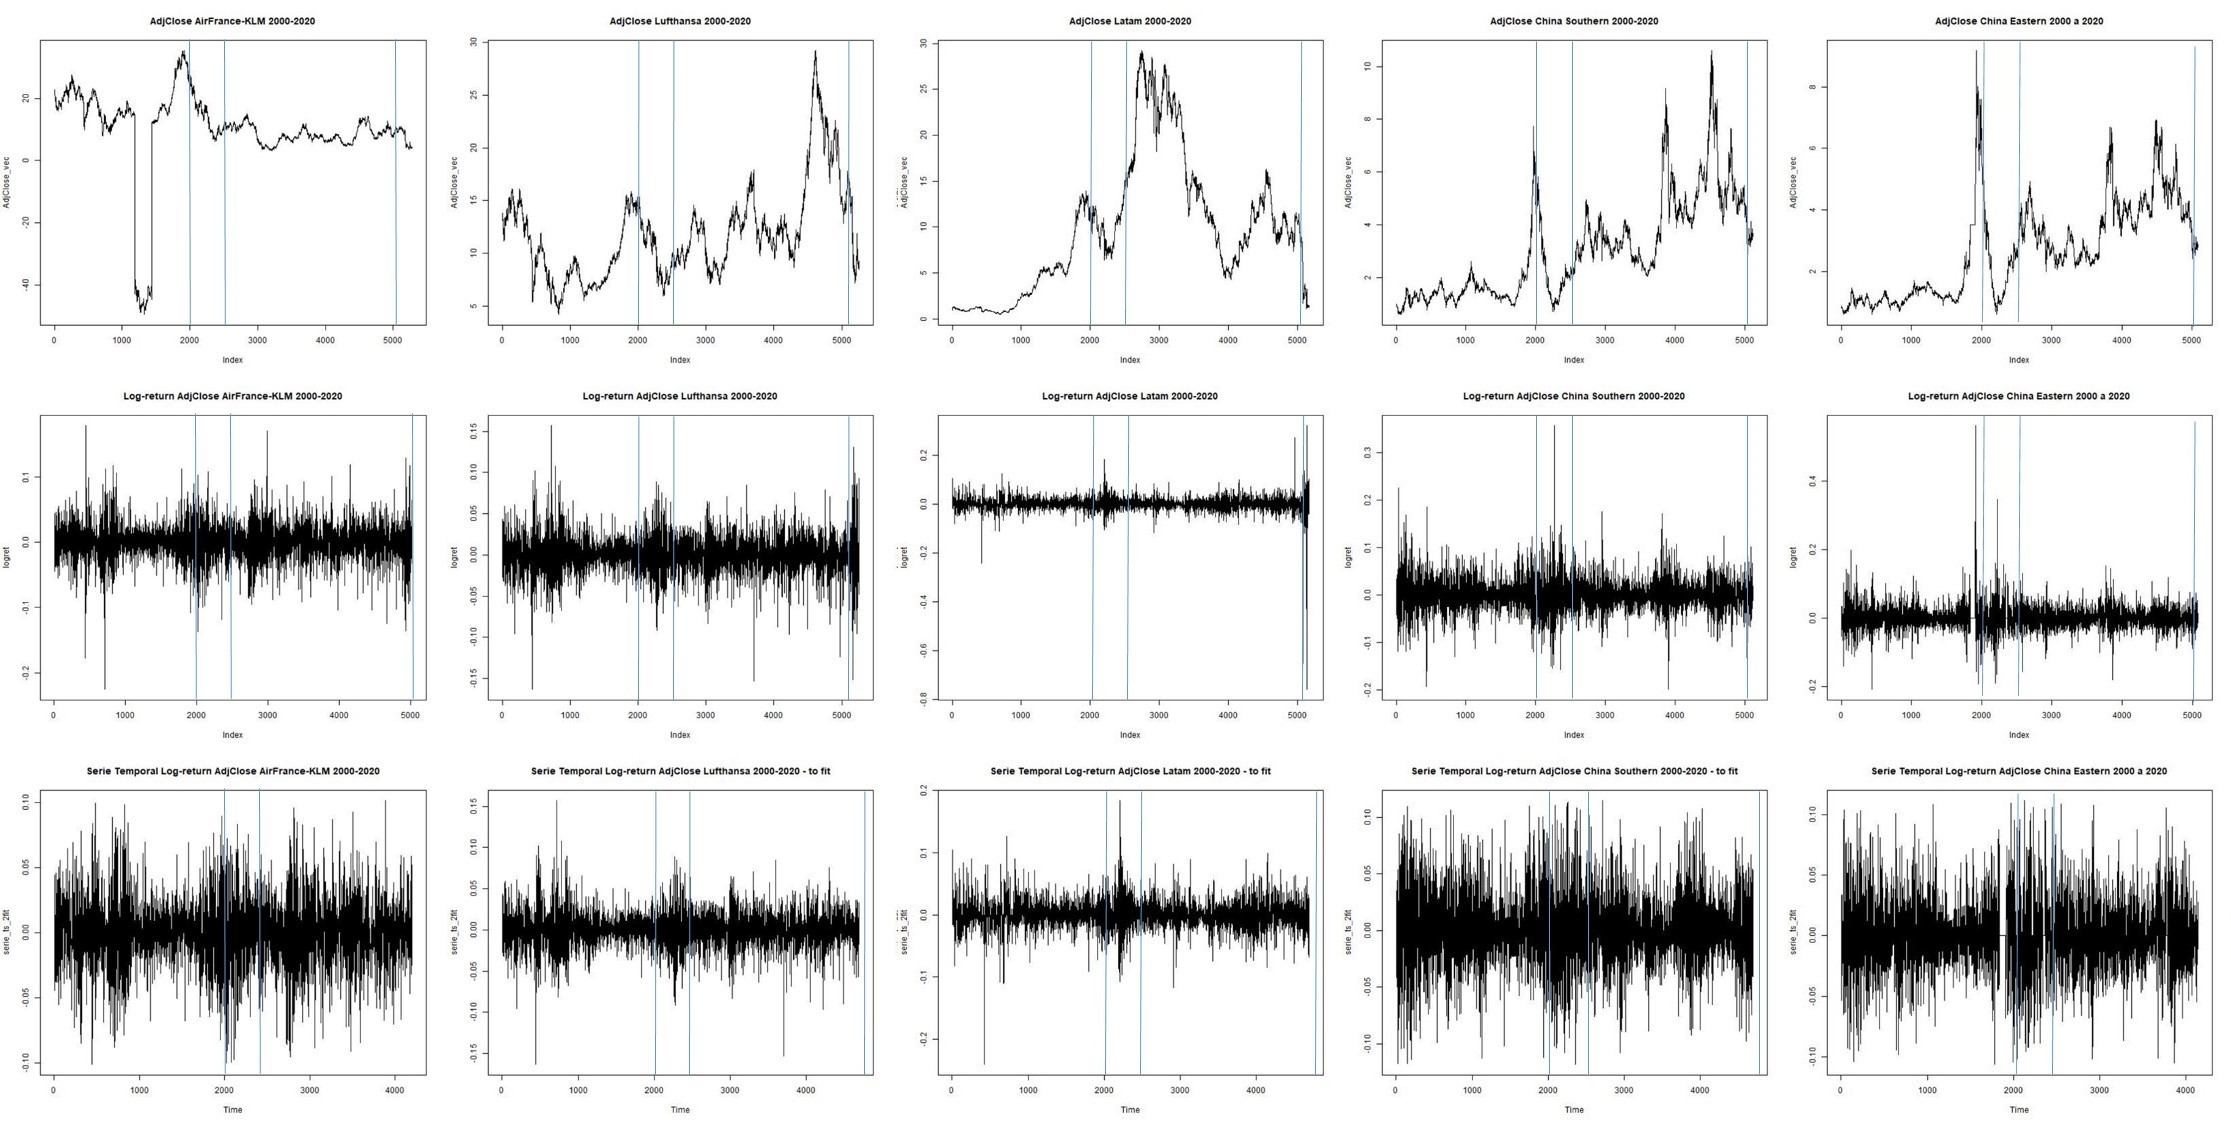
\includegraphics[width=1.0\linewidth]{../Modelos/CompGeral00a20}
	\caption{Gráficos Comparativos - Preços Ajustados, Log-Return, Série Temporal do Log-Return}
	\label{fig:compgeral00a20}
\end{figure}

Em todas as companhias existe a queda abrupta no primeiro gráfico, como previsto. Consequentemente, deve haver algum efeito observável nas séries do \textit{log-return}, exibidas na figura \ref{fig:compgeral00a20} nos segundos e terceiros gráficos. De fato, o efeito produzido é percebido em forma de picos, tanto positivos quanto negativos. Repare que entre as linhas azuis, isto é, entre 2008 e 2009, há um grande grau de volatilidade nessas séries, haja vista esse comportamento mais acentuado. Tal mudança drástica se dá devido à natureza do \textit{log-return}, pois, como expresso na equação \ref{eq_logret}, esse retorno computa as diferenças entre os valores das ações no tempo $t$ e $t-1$. Sendo assim, é trivial o fato de quedas abruptas nos preços terem como consequência picos acentuados no \textit{log-return}. Apenas no caso da \textit{AirFrance-KLM} este fato não é tão perceptível. Para fins de ajuste de modelos $ARIMA$, esses picos de volatilidade são muito indesejáveis, uma vez que não correspondem à evolução natural da série. É por esse motivo que choques externos são imprevisíveis ao olharmos apenas para a série estudada e, além disso,  tornam o desenvolvimento dela também de difícil previsão. 

Ao mesmo tempo em que a queda de preços foi abrupta, a recuperação não tardou muito a ocorrer. A principal estratégia para contornar uma crise como a de 2008 é tentar reanimar a economia, ou seja, criar maneiras de movimentar e reiniciar as transações econômicas em suas diferentes escalas. Para tal, uma primeira ação clássica é aplicar uma redução de juros para injetar dinheiro na economia e incentivar o consumo e investimento que, por sua vez, incentivam a produção. Caso este método se mostre insuficiente, uma solução é, assim como foi descoberto em 2008, realizar um socorro púbico às empresas de caráter privado. Nesse sentido, o governo, ao invés de passar pelo intermédio dos bancos, que em uma crise podem reter recursos com receio de quebra, injeta capital de forma direta nas empresas. Em maiores detalhes, foi esta a estratégia, denominada \textit{Quantitative Easing - QE} adotada pelos Bancos Centrais em 2008, que passaram a comprar títulos de dívida de empresas privadas, aumentando o volume de capital em circulação e garantindo liquidez para o mercado que estava congelado. 

Feita esta análise, olhemos para a terceira linha azul nos gráficos da figura \ref{fig:compgeral00a20}, que indica o início do ano de 2020. Novamente é possível perceber a queda nos preços das ações das companhias aéreas que, da mesma forma visualizada em 2008, traduz-se em picos de volatilidade nas séries do \textit{log-return}. Por outro lado, existem algumas diferenças consideráveis entre a crise anterior e a gerada pela Covid-19. Primeiramente, enquanto aquela teve como origem o próprio mercado financeiro, esta configura-se como um choque inteiramente externo ao mercado, tornando-o ainda mais invisível aos modelos de econometria. Em segundo lugar, enquanto em 2008 o mercado congelou suas atividades de forma espontânea, em 2020, novamente, a parada de diversas atividades econômicas ocorreu como consequência de ordens externas. A principal diferença, no entanto, é que ainda vivemos a crise da Covid-19, tornando-nos incapazes de analisar com precisão seus reais efeitos a médio e longo prazo. É certo que o \textit{Quantitative Easing} está sendo utilizado, fruto de seu bom funcionamento no passado, tornando-se mais uma estratégia importante no combate à instabilidade econômica. O \textit{U.S Federal Reserve}, por exemplo anunciou um programa de \textit{QE} de mais de 700 bilhões de dólares. Há aqueles que consideram que esta estratégia, aprendida em 2008, causará uma recuperação mais rápida para os efeitos negativos da crise de 2020, no entanto, possíveis segundas ondas de contaminação, possibilidade de novas medidas de contenção e um enorme medo por parte da sociedade tornam, ao meu ver, essa previsão pouco confiável.
 
\subsubsection{Ajuste e previsão de modelos ARIMA}\label{subsec_for}
Nesta seção serão apresentados os resultados obtidos da aplicação dos métodos discutidos na seção \ref{subsec_R}, tendo como dados de entrada os preços ajustados das ações de dez companhias aéreas, enumeradas na seção \ref{subsec_crise}. Dito isso, foi feito o ajuste para modelos $ARIMA$ de todas as empresas no período de 2010 a 2019, reservando uma parte da série para validação e comparação dos modelos com os valores reais. A imagens \ref{fig:seriescompusa1019} a \ref{fig:seriescompeuropa1019} exibem, simultaneamente, os preços ajustados das ações das companhias aéreas e a série temporal do \textit{log-return} destes preços, após os devidos tratamentos já apresentados.

\begin{figure}[H]
	\centering
	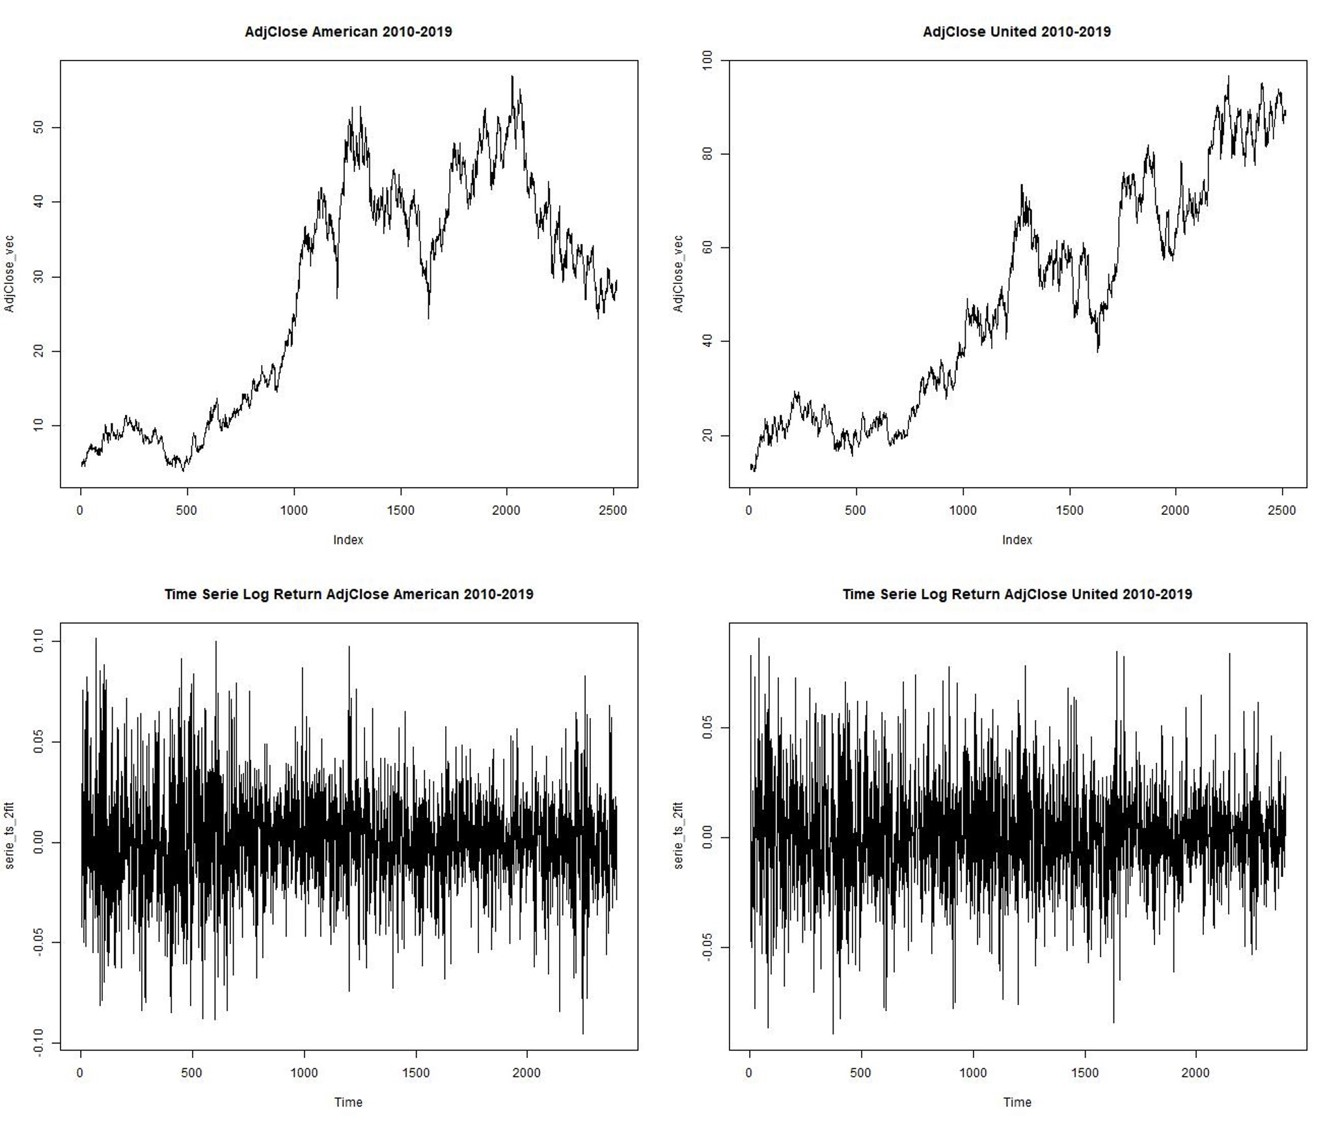
\includegraphics[width=0.8\linewidth]{../Modelos/SeriesCompUSA10_19}
	\caption{Preços ajustados e Log Return - American e United}
	\label{fig:seriescompusa1019}
\end{figure}

\begin{figure}[H]
	\centering
	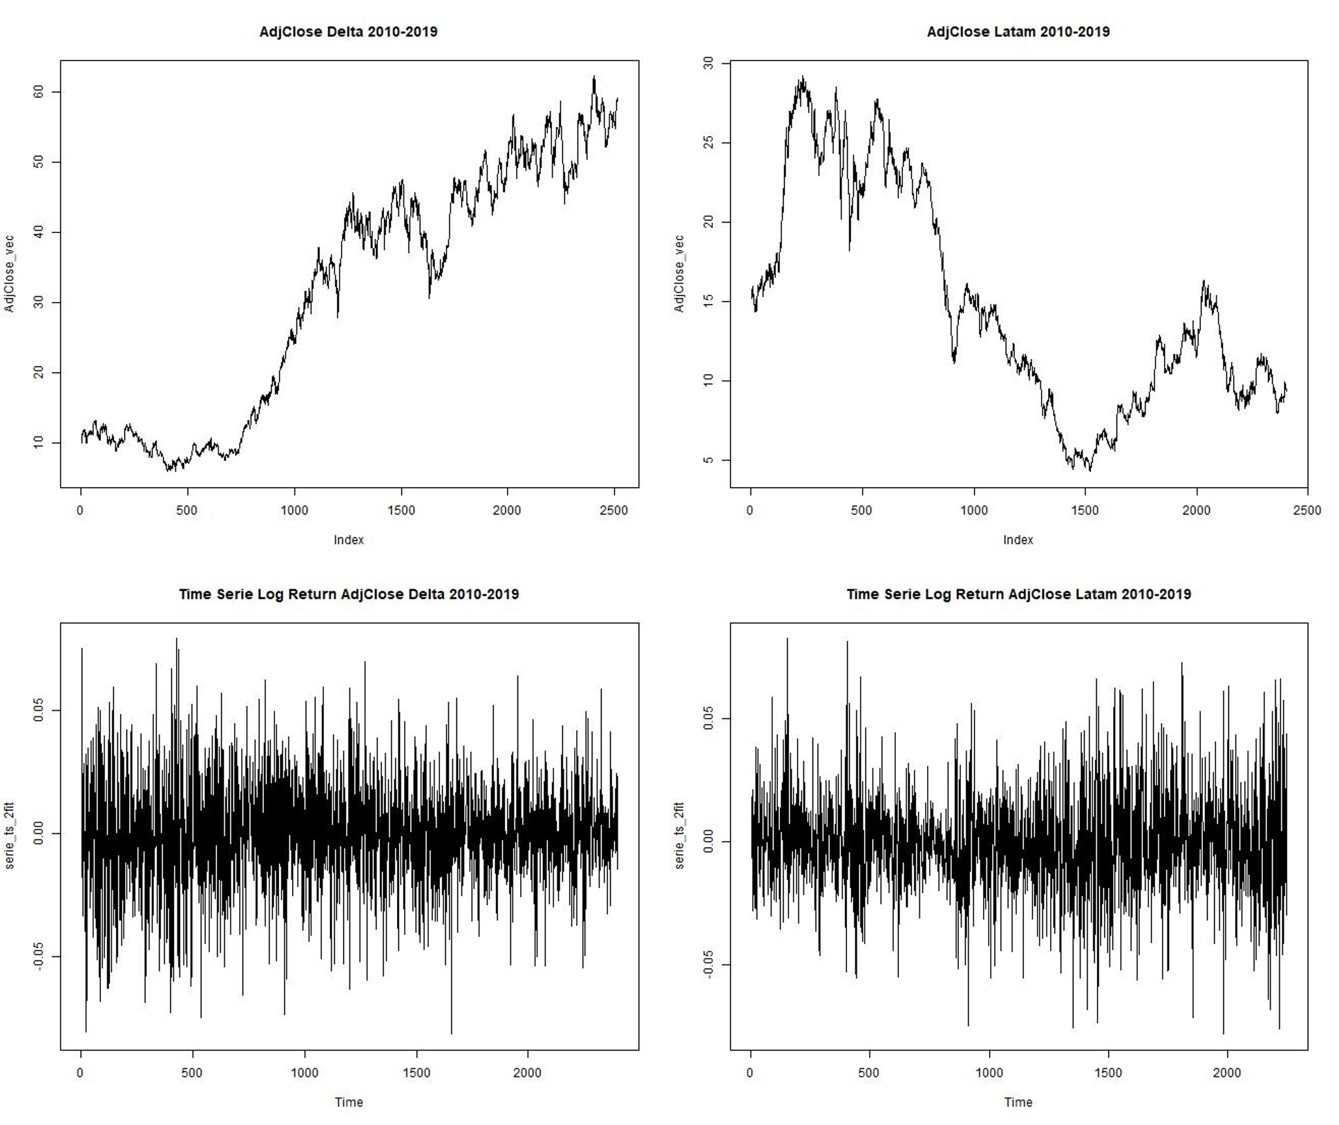
\includegraphics[width=0.8\linewidth]{../Modelos/SeriesCompDeltaLat10_19}
	\caption{Preços ajustados e Log Return - Delta e Latam}
	\label{fig:seriescompdeltalat1019}
\end{figure}

\begin{figure}[H]
	\centering
	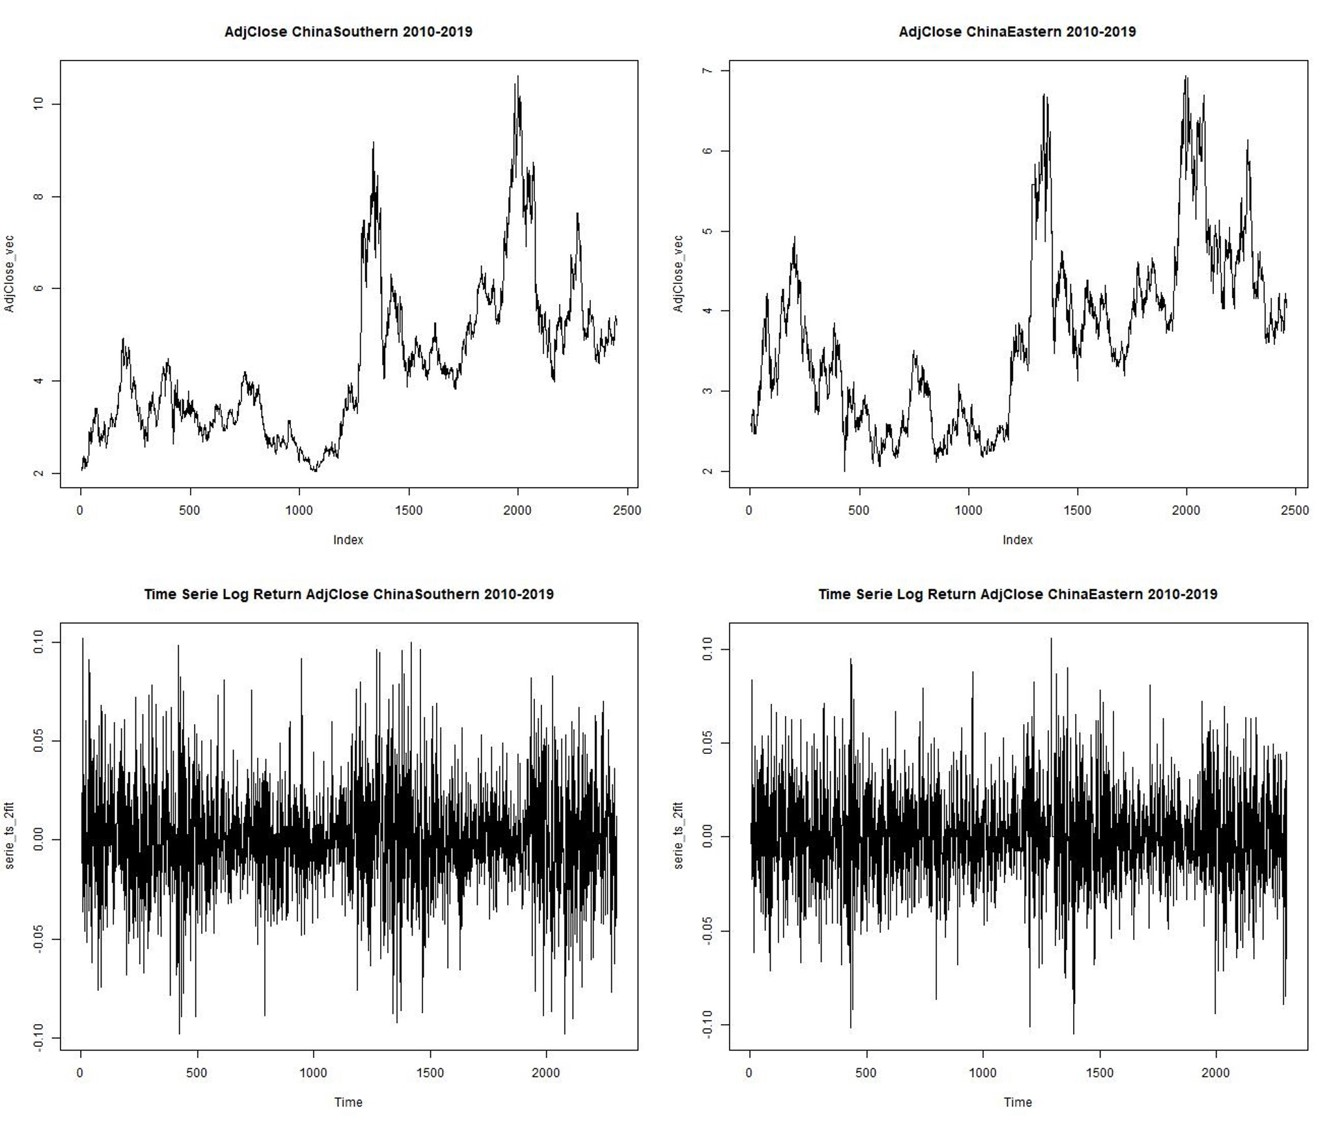
\includegraphics[width=0.8\linewidth]{../Modelos/SeriesCompChina10_19}
	\caption{Preços ajustados e Lo Return - China Southern e China Eastern}
	\label{fig:seriescompchina1019}
\end{figure}

\begin{figure}[H]
	\centering
	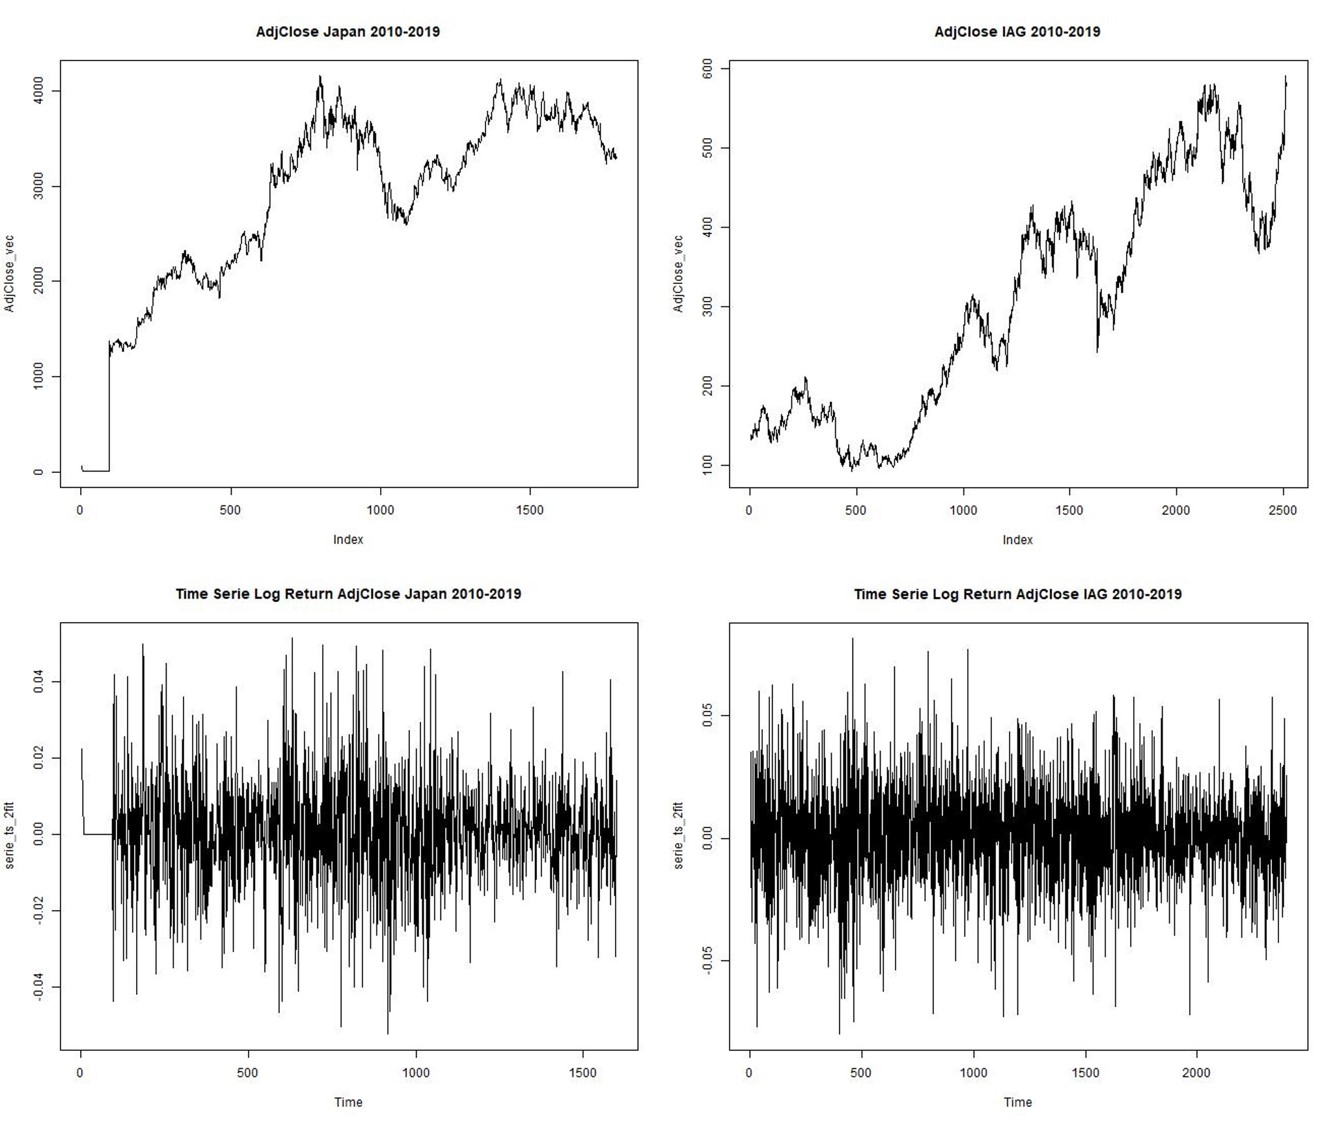
\includegraphics[width=0.8\linewidth]{../Modelos/SeriesCompJapIAG10_19}
	\caption{Preços ajustados e Log Return - Japan e IAG}
	\label{fig:seriescompjapiag1019}
\end{figure}

\begin{figure}[H]
	\centering
	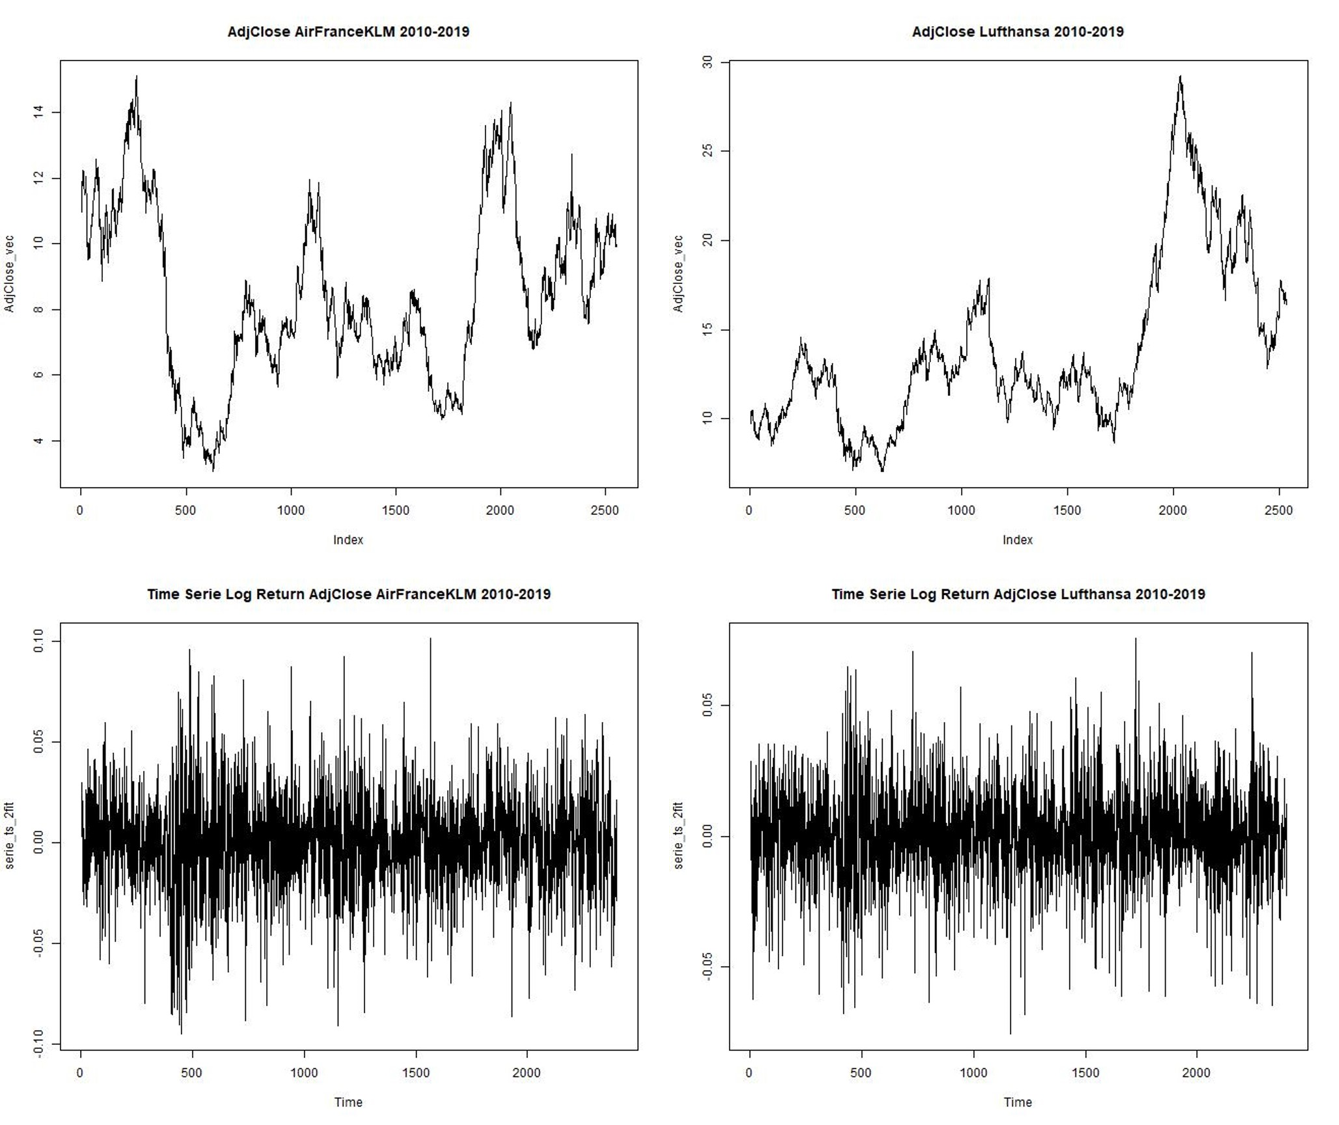
\includegraphics[width=0.8\linewidth]{../Modelos/SeriesCompEuropa10_19}
	\caption{Preços ajustados e Log Return - AirFrance KLM e Lufthansa}
	\label{fig:seriescompeuropa1019}
\end{figure}

Uma vez visualizadas as séries, foram executados ambos \textit{Augmented Dickey-Fuller Test} e o teste para sazonalidade, via métodos $adf.test()$ e $decompose()$. O \textit{output} da execução do primeiro encontra-se abaixo:
\begin{gather*}
Augmented Dickey-Fuller Test\\
data:  serie.ts.2fit\\
Dickey-Fuller = -12.924, Lag Order = 13, p-value = 0.01\\
alternative hypothesis: stationary\\
\end{gather*}

Para todas as séries analisadas, este método retornou \emph{p-values} iguais ou menores que $0.01$, o que demonstra, no máximo, $1\%$ de probabilidade de existir uma raiz unitária no polinômio característico das séries. Devido a isso, omite-se o resultado das demais séries, que são encontrados em \cite{git}. Consequentemente, todos os \textit{log-returns} estudados apresentam aspecto estacionário. O método $decompose()$ também apresentou retornos similares para todas as séries, sendo este a seguinte mensagem de erro: \emph{Error in decompose(serieTs2fit): série temporal não tem período, ou tem menos de 2}. Isto quer dizer que os retornos das ações das companhias aéreas não possuem perfil sazonal, o que pode ser contra intuitivo, haja vista o claro comportamento sazonal de viagens aéreas, mais intensas em períodos de férias escolares, por exemplo. Desse modo, a perda de sazonalidade entre as viagens em si e os retornos dos ativos indica um grau de maturidade do mercado de ações dessas companhias, sendo capaz de suavizar seu perfil sazonal. É interessante, no entanto, suspeitar que uma mudança na escala temporal da análise pode ter como consequência o aparecimento de ciclos sazonais, algo que será objetivo de análise futura, após introduzido o ferramental das \emph{ondaletas}. 

Uma vez confirmado o caráter estacionário e não sazonal das séries a serem ajustadas, tornamo-nos aptos a analisar as funções de correlação já conhecidas, $ACF$ e $PACF$. Utilizando os métodos apresentados na seção \ref{subsec_R}, foram produzidos os seguintes correlogramas. 

\begin{figure}[H]
	\centering
	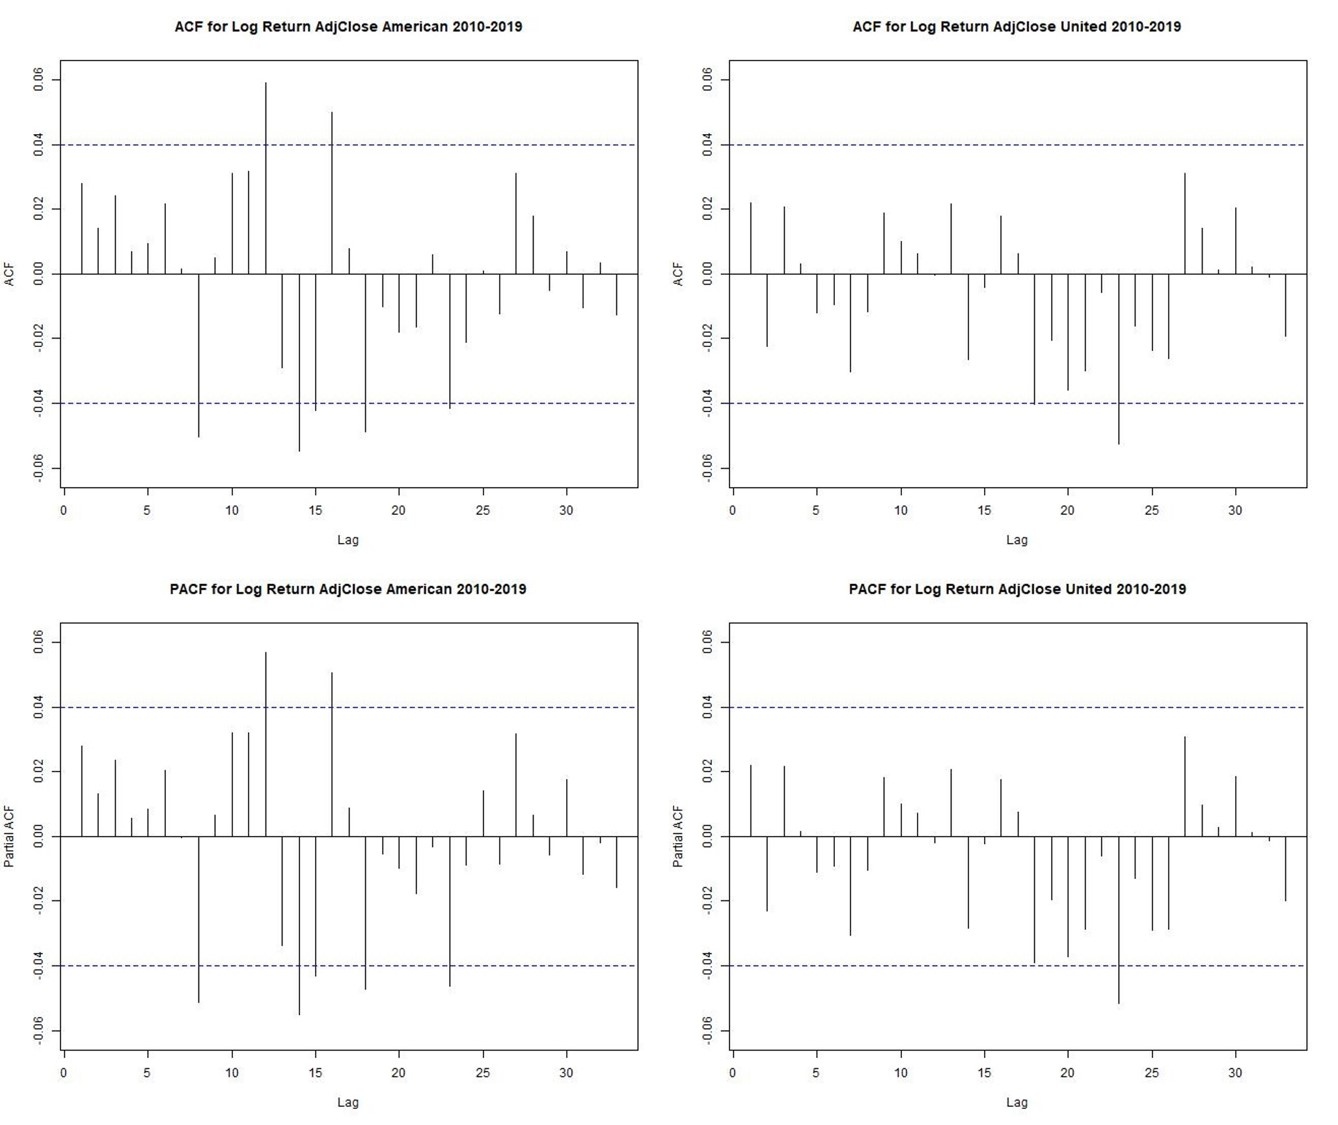
\includegraphics[width=0.8\linewidth]{../Modelos/CorrelationsUSA10_19}
	\caption{ACF e PACF - American e United}
	\label{fig:correlationsusa1019}
\end{figure}

\begin{figure}[H]
	\centering
	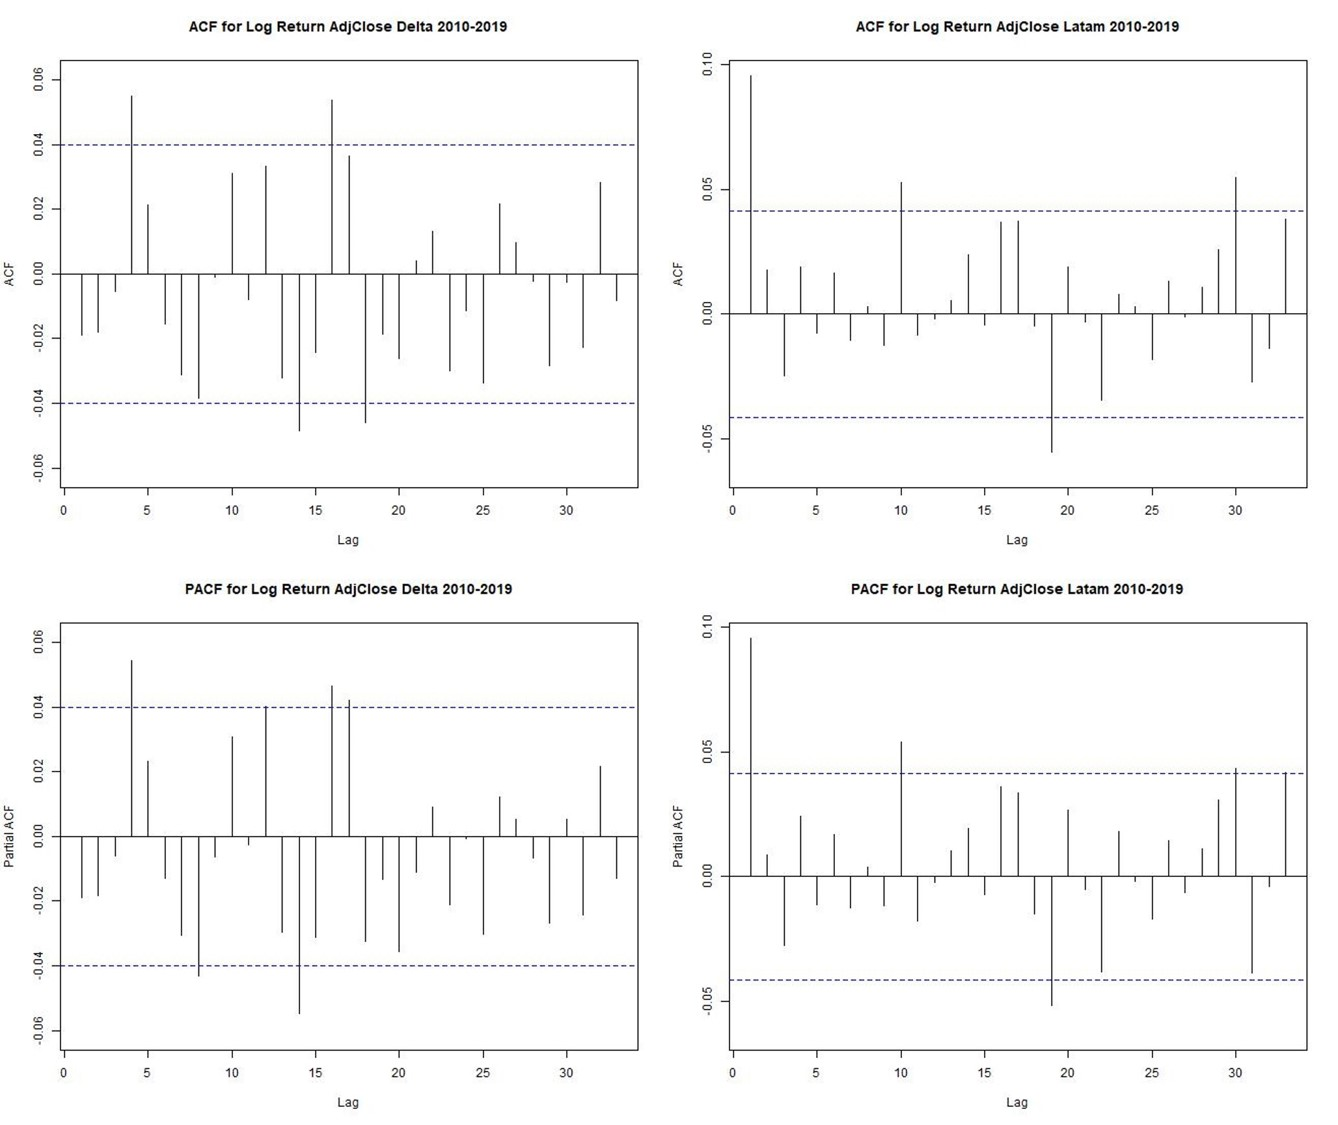
\includegraphics[width=0.8\linewidth]{../Modelos/CorrelationsDeltaLat10_19}
	\caption{ACF e PACF - Delta e Latam}
	\label{fig:correlationsdeltalat1019}
\end{figure}

\begin{figure}[H]
	\centering
	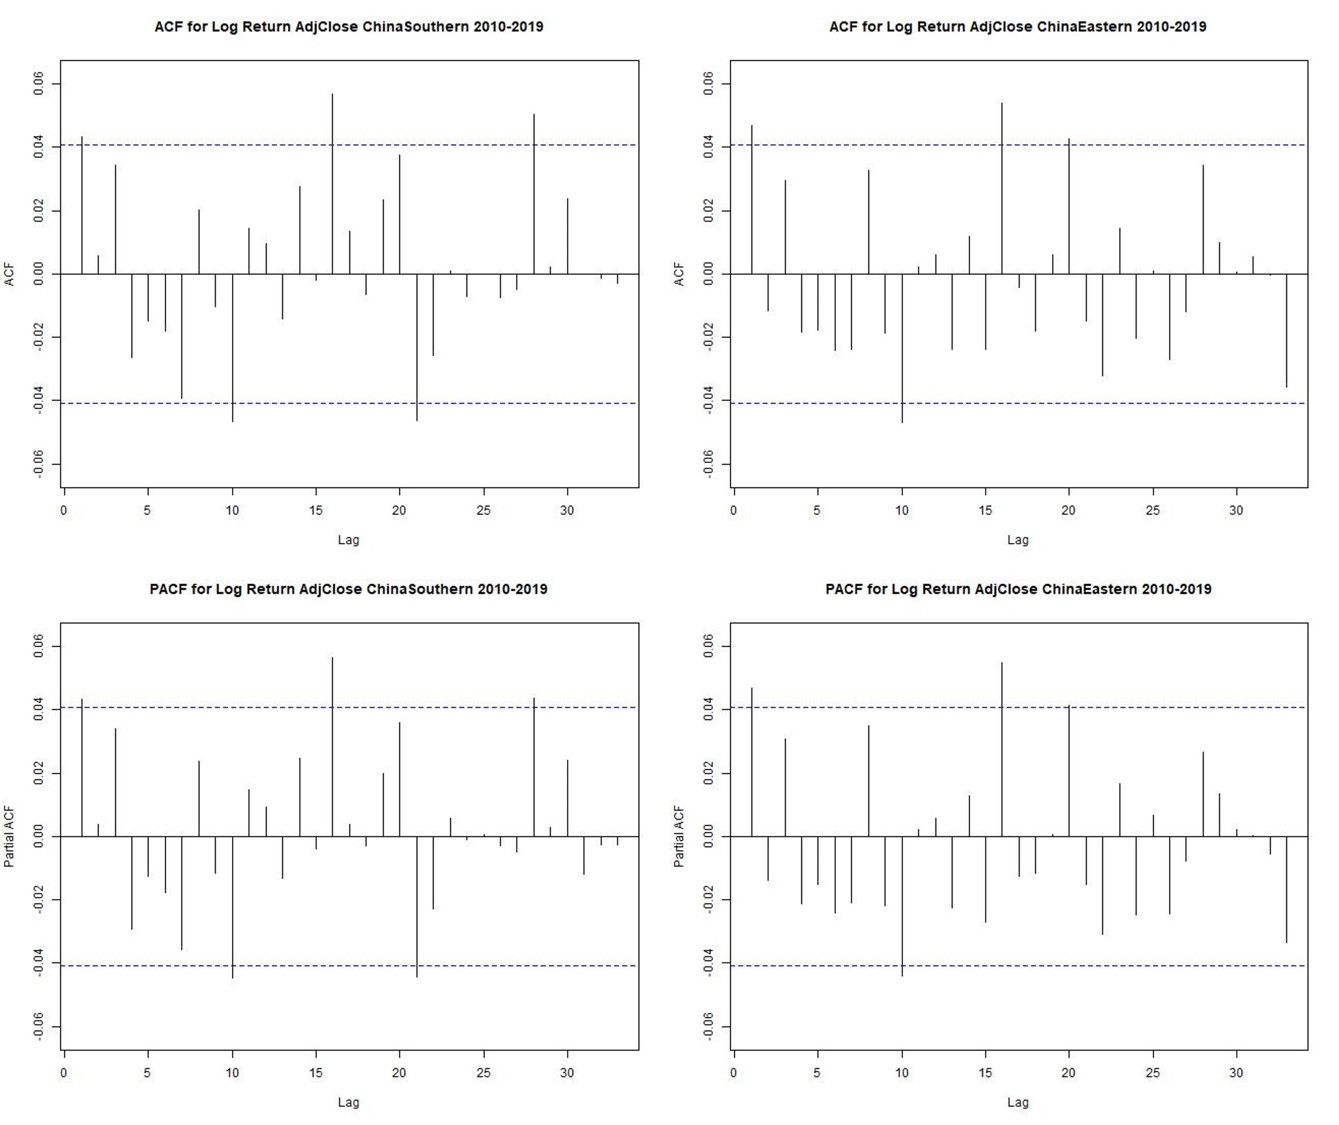
\includegraphics[width=0.8\linewidth]{../Modelos/CorrelationsChina10_19}
	\caption{ACF e PACF - China Southern e China Eastern}
	\label{fig:correlationschina1019}
\end{figure}

\begin{figure}[H]
	\centering
	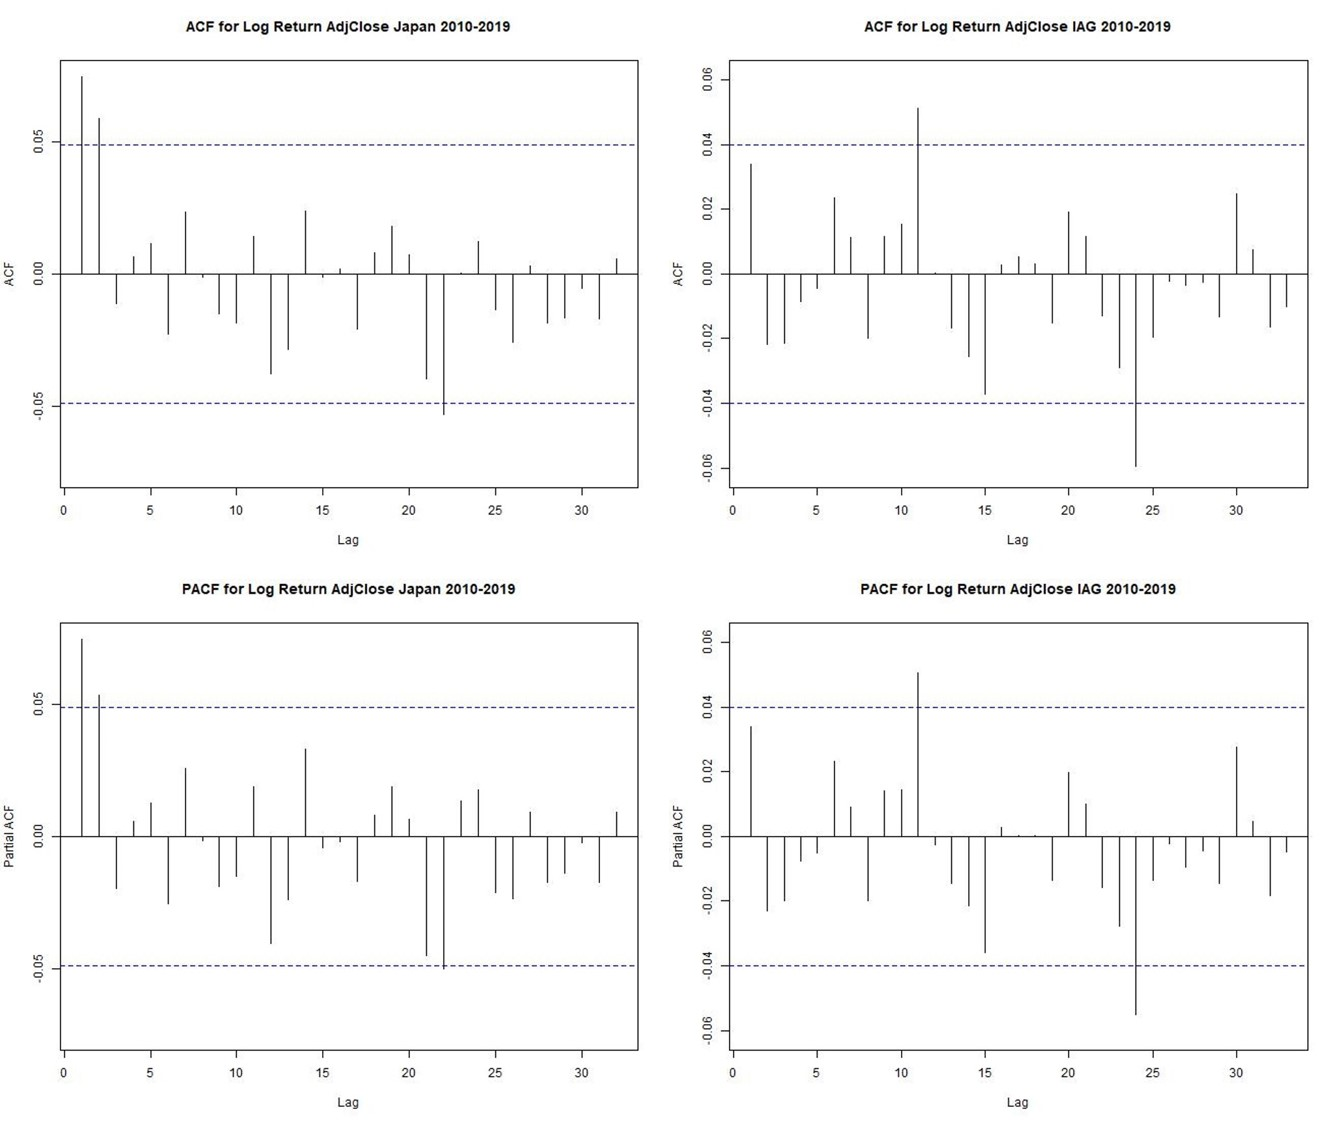
\includegraphics[width=0.8\linewidth]{../Modelos/CorrelationsJapanIAG10_19}
	\caption{ACF e PACF - Japan e IAG}
	\label{fig:correlationsjapaniag1019}
\end{figure}

\begin{figure}[H]
	\centering
	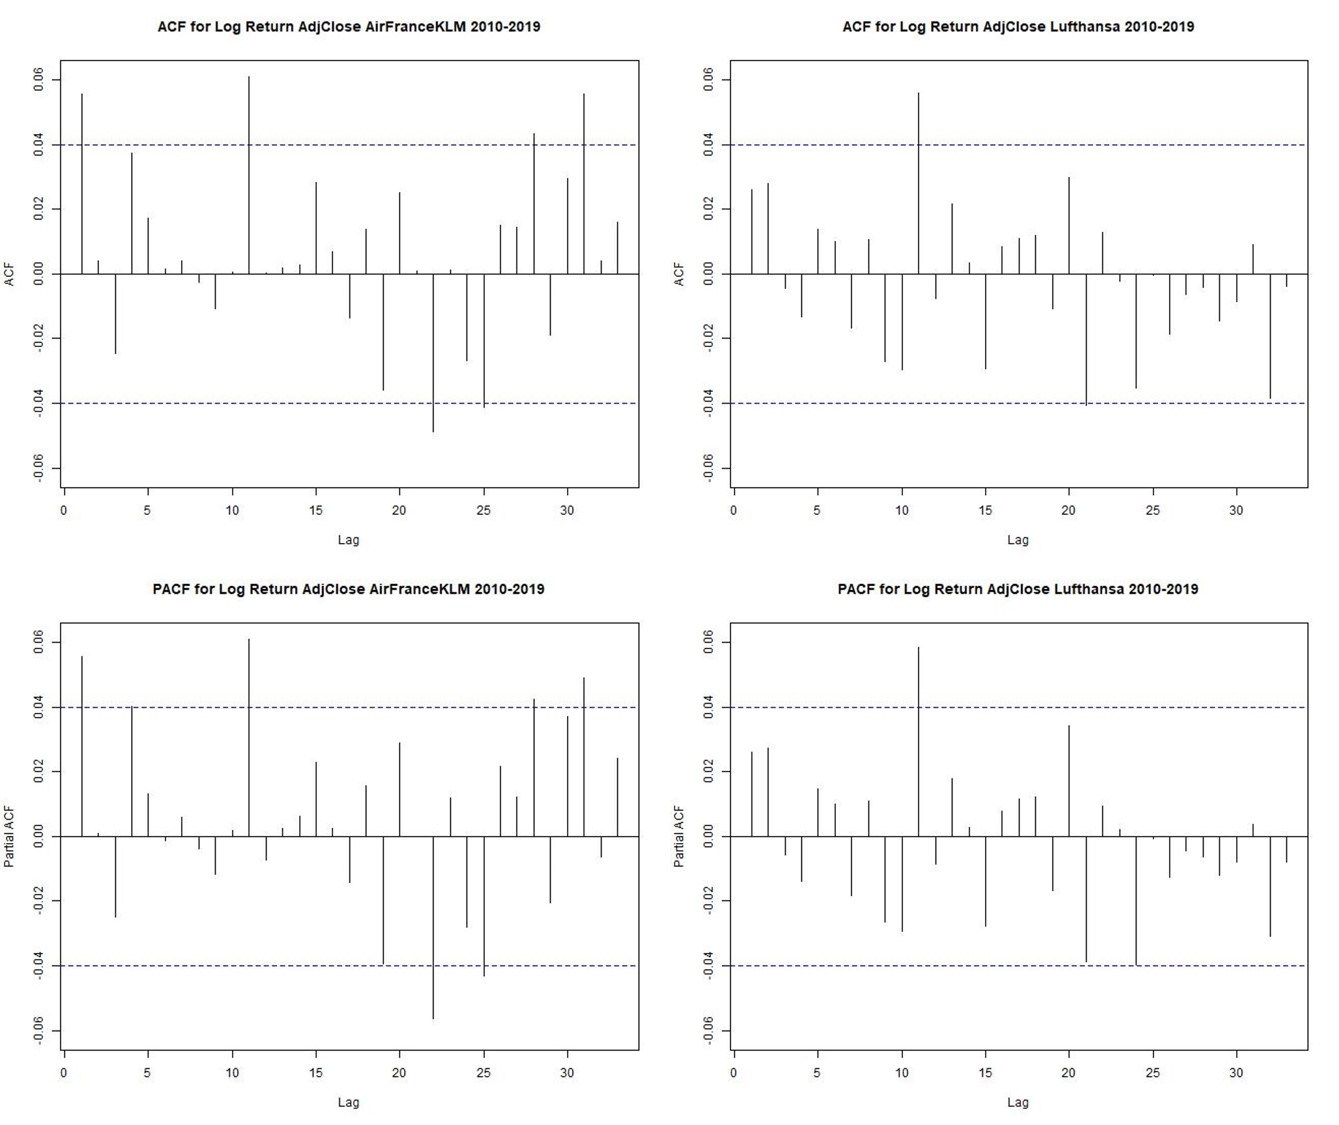
\includegraphics[width=0.8\linewidth]{../Modelos/CorrelationsAirKLM10_19}
	\caption{ACF e PACF - AriFrance-KLM e Lufthansa}
	\label{fig:correlationsairklm1019}
\end{figure}

A interpretação dos gráficos presentes nas figuras \ref{fig:correlationsusa1019} a \ref{fig:correlationsairklm1019} é, de certo modo, trivial. Como apresentado na seção \ref{subsec_R}, procuramos os \textit{lags} estatisticamente não nulos, isto é, acima da linha pontilhada superior ou abaios da inferior dos gráficos. Dessa forma, foram ajustados os seguintes modelos $ARIMA(p,d,q)$ para cada companhia aérea: \emph{\textbf{American} - (8,0,0), (0,0,8), (12,0,0), (0,0,12), (14,0,0), (0,0,14), (8,0,8), (12,0,8) e (14,0,8); \textbf{United} - (23,0,0), (0,0,23); \textbf{Delta} - (4,0,0), (0,0,4), (0,0,8), (4,0,4); \textbf{Latam} - (1,0,0), (0,0,1), (10,0,0), (0,0,10), (19,0,0), (0,0,19), (1,0,1), (1,0,10), (1,0,19), (10,0,1); \textbf{China Southern} - (1,0,0), (0,0,1), (10,0,0), (0,0,10), (16,0,0), (0,0,16), (1,0,1), (1,0,10), (1,0,16), (10,0,1), (16,0,1); \textbf{China Eastern} - (1,0,0), (0,0,1), (10,0,0), (0,0,10), (16,0,0), (0,0,16), (1,0,1), (1,0,10), (1,0,16), (10,0,1), (10,0,16), (16,0,1); \textbf{Japan} - (1,0,0), (0,0,1), (2,0,0), (0,0,2), (1,0,1), (1,0,2), (2,0,1), (2,0,2); \textbf{IAG} - (1,0,0), (0,0,1), (11,0,0), (0,0,11), (24,0,0), (0,0,24), (1,0,1), (1,0,11), (1,0,24), (11,0,1), (11,0,24), (24,0,1); \textbf{AirFrance KLM} - (1,0,1), (0,0,1), (11,0,0), (0,0,11), (0,0,21), (1,0,1), (1,0,11), (1,0,21), (11,0,1), (11,0,11), (21,0,1) e \textbf{Lufthansa} - (11,0,0), (0,0,11), (21,0,0)}.

Uma vez ajustados todos os inúmeros modelos, torna-se essencial compará-los a fim de selecionar os mais adequados. Para tal, é feita uma análise envolvendo duas medidas estatísticas, o \textit{log likelihood} e o \textit{aic}. Suas interpretações se dão de modo que o \textit{log likelhood} deve ser o maior possível, enquano o \textit{aic} o menor possível. Com base nessas medidas, foram selecionados de dois modelos $ARIMA$ de cada companhia aérea para serem calculadas as previsões dos retornos de seus ativos. Os modelos selecionados foram: \emph{\textbf{American} - (12,0,8) e (14,0,8); \textbf{United} - (23,0,0) e (23,0,23); \textbf{Delta} - (0,0,4) e (4,0,4); \textbf{Latam} - (1,0,0) e (1,0,19); \textbf{China Southern} - (1,0,0) e (16,0,1); \textbf{China Eastern} - (10,0,16) e (0,0,1); \textbf{Japan} - (0,0,2) e (2,0,2); \textbf{IAG} - (1,0,0) e (11,0,24); \textbf{AirFrance KLM} - (1,0,0) e (11,0,11) e \textbf{Lufthansa} - (11,0,0)} e (21,0,0). Com o intuito de não poluir este relatório, serão exibidos a seguir os coeficientes e outras medidas importantes apenas dos melhores modelos de cada companhia, com base em seus \textit{log likelihood} e \textit{aic}. No entanto, todas as informações produzidas que não estão exibidas encontram-se em \cite{git}.

\begin{table}[H]
\centering
\begin{tabular}{|l|l|l|l|l|l|l|l|l|l|}
\hline
ar1    & ar2     & ar3     & ar4    & ar5     & ar6     & ar7     & ar8    & ar9    & ar10   \\ \hline
0.0875 & -0.2647 & -0.0537 & 0.3572 & -0.1591 & -0.0099 & -0.0805 & -0.643 & 0.0241 & 0.0176 \\ \hline
ar11   & ar12    & ma1     & ma2    & ma3     & ma4     & ma5     & ma6    & ma7    & ma8    \\ \hline
0.0326 & 0.0872  & -0.0641 & 0.2853 & 0.0864  & -0.3499 & 0.1658  & 0.0334 & 0.0947 & 0.6223 \\ \hline
\multicolumn{10}{|c|}{loglikelihood = 5349.78}                                               \\ \hline
\multicolumn{10}{|c|}{aic = -10655.56}                                                       \\ \hline 
\end{tabular}
\caption{Coeficientes American - ARIMA(12,0,8)}
\label{tab:American1208}
\end{table}

\begin{table}[H]
	\centering
	\begin{tabular}{|l|l|l|l|l|l|l|l|l|l|}
		\hline
		ar1    & ar2    & ar3     & ar4     & ar5     & ar6     & ar7     & ar8     & ar9     & ar10   \\ \hline
		0.1518 & 0.022  & -0.0951 & 0.4539  & -0.0262 & -0.2079 & -0.0159 & -0.6647 & 0.0316  & 0.0259 \\ \hline
		ar11   & ar12   & ar13    & ar14    & ma1     & ma2     & ma3     & ma4     & ma5     & ma6    \\ \hline
		0.0216 & 0.0826 & -0.0182 & -0.0535 & -0.1288 & -0.0027 & -0.1207 & -0.4531 & -0.0188 & 0.2193 \\ \hline
		ma7    & ma8    & \multicolumn{8}{l|}{}                                                        \\ \hline
		0.0207 & 0.6281 & \multicolumn{8}{l|}{}                                                        \\ \hline
		\multicolumn{10}{|c|}{loglikelihood = 5350.57}                                                 \\ \hline
		\multicolumn{10}{|c|}{aic = -10653.15}                                                         \\ \hline
	\end{tabular}
\caption{Coeficientes American - ARIMA(14,0,8)}
\label{tab:American1408}
\end{table}

\begin{table}[H]
	\centering
	\begin{tabular}{|l|l|l|l|}
		\hline
		ma1        & ma2        & ma3       & ma4      \\ \hline
		-0.0219    & -0.0146    & 0.0001    & 0.0607   \\ \hline
		\multicolumn{4}{|c|}{Log Likelihood = 5844.54} \\ \hline
		\multicolumn{4}{|c|}{aic = -11667.07}          \\ \hline
	\end{tabular}
\caption{Coeficientes Delta - ARIMA(0,0,4)}
\label{tab:Delta004}
\end{table}

\begin{table}[H]
	\centering
	\begin{tabular}{|l|l|l|l|l|l|l|l|}
		\hline
		ar1   & ar2    & ar3     & ar3    & ma1     & ma2    & ma3    & ma4     \\ \hline
		0.400 & -0.225 & -0.5555 & 0.1122 & -0.4251 & 0.2224 & 0.5638 & -0.0684 \\ \hline
		\multicolumn{8}{|c|}{Log Likelihood = 5854}                             \\ \hline
		\multicolumn{8}{|c|}{aic = -11688.01}                                   \\ \hline
	\end{tabular}
\caption{Coeficientes Delta - ARIMA(4,0,4)}
\label{tab:Delta404}
\end{table}

\begin{table}[H]
	\centering
	\begin{tabular}{|c|}
		\hline
		ar1                      \\ \hline
		0.0957                   \\ \hline
		Log Likelihood = 5599.05 \\ \hline
		aic = -11192.11          \\ \hline
	\end{tabular}
\caption{Coeficientes Latam - ARIMA(1,0,0)}
\label{tab:Latam100}
\end{table}

\begin{table}[H]
	\centering
	\begin{tabular}{|l|l|l|l|l|l|l|l|l|l|}
		\hline
		ar1    & ma1    & ma2     & ma3     & ma4     & ma5    & ma6     & ma7     & ma8     & ma9   \\ \hline
		-0.1615 & 0.2599  & 0.0402 & -0.0268  & 0.0102 & -0.0003 & 0.0126 & -0.009  & 0.0064  & -0.0128 \\ \hline
		ma10   & ma11   & ma12    & ma13    & ma14     & ma15     & ma16     & ma17     & ma18     & ma19    \\ \hline
		0.0484 & 0.0078 &-0.0034 & -0.007 & 0.0272 & 0.0019 & 0.0247 & 0.0427 & 0.0016 & -0.0648 \\ \hline
		\multicolumn{10}{|c|}{loglikelihood = 5612.51}                                                 \\ \hline
		\multicolumn{10}{|c|}{aic = -11181.01}                                                         \\ \hline
	\end{tabular}
	\caption{Coeficientes Latam - ARIMA(1,0,19)}
	\label{tab:Latam1019}
\end{table}

\begin{table}[H]
	\centering
	\begin{tabular}{|c|}
		\hline
		ar1                      \\ \hline
		0.0434                   \\ \hline
		Log Likelihood = 5030.81 \\ \hline
		aic = -10055.62          \\ \hline
	\end{tabular}
\caption{Coeficientes China Southern - ARIMA(1,0,0)}
\label{tab:ChinaSouth100}
\end{table}

\begin{table}[H]
	\centering
	\begin{tabular}{|l|l|l|l|l|l|l|l|l|l|}
		\hline
		ar1    & ar2     & ar3     & ar4     & ar5     & ar6     & at7     & \multicolumn{1}{l|}{ar8}    & \multicolumn{1}{l|}{ar9}     & \multicolumn{1}{l|}{ar10}    \\ \hline
		0.1138 & -0.0011 & 0.0325  & -0.0291 & -0.0113 & -0.0147 & -0.032  & \multicolumn{1}{l|}{0.0252} & \multicolumn{1}{l|}{-0.0095} & \multicolumn{1}{l|}{-0.0430} \\ \hline
		ar11   & ar12    & ar13    & ar14    & ar15    & ar16    & ma1     &                             &                              &                              \\ \hline
		0.0176 & 0.0106  & -0.0174 & 0.0264  & -0.0088 & 0.0573  & -0.0693 &                             &                              &                              \\ \hline
		\multicolumn{10}{|c|}{Log Likelihood = 5043.31}                                                                                                                \\ \hline
		\multicolumn{10}{|c|}{aic = -10048.61}                                                                                                                         \\ \hline
	\end{tabular}
\caption{Coeficientes China Southern - ARIMA(16,0,1)}
\label{tab:ChinaSouth1601}
\end{table}

\begin{table}[H]
	\centering
	\begin{tabular}{|c|}
		\hline
		ma1                      \\ \hline
		0.0484                   \\ \hline
		Log Likelihood = 5113.95	 \\ \hline
		aic = -10221.91          \\ \hline
	\end{tabular}
	\caption{Coeficientes China Eastern - ARIMA(0,0,1)}
	\label{tab:ChinaEast001}
\end{table}

\begin{table}[H]
	\centering
	\begin{tabular}{|l|l|}
		\hline
		ma1                    & ma2                   \\ \hline
		0.0727                 & 0.0604                \\ \hline
		\multicolumn{2}{|c|}{Log Likelihood = 4549.41} \\ \hline
		\multicolumn{2}{|c|}{aic = -9090.83}           \\ \hline
	\end{tabular}
\caption{Coeficientes Japan - ARIMA(0,0,2)}
\label{tab:Japan002}
\end{table}

\begin{table}[H]
	\centering
	\begin{tabular}{|l|l|l|l|}
		\hline
		ma1        & ar2        & ma1      & ma2      \\ \hline
		-0.2099    & -0.0255    & 0.282    & 0.1005   \\ \hline
		\multicolumn{4}{|c|}{Log Likelihood = 4549.6} \\ \hline
		\multicolumn{4}{|c|}{aic = -9087.19}          \\ \hline
	\end{tabular}
\caption{Coeficientes Japan - ARIMA(2,0,2)}
\label{tab:Japan202}
\end{table}

\begin{table}[H]
	\centering
	\begin{tabular}{|c|}
		\hline
		ar1                      \\ \hline
		0.0341                   \\ \hline
		Log Likelihood = 5931.49	 \\ \hline
		aic = -11856.97          \\ \hline
	\end{tabular}
	\caption{Coeficientes IAG - ARIMA(1,0,0)}
	\label{tab:IAG100}
\end{table}

\begin{table}[H]
	\centering
	\begin{tabular}{|c|}
		\hline
		ar1                      \\ \hline
	    0.0557                   \\ \hline
		Log Likelihood = 5478.34	 \\ \hline
		aic = -10950.67          \\ \hline
	\end{tabular}
	\caption{Coeficientes KLM - ARIMA(1,0,0)}
	\label{tab:KLM100}
\end{table}

Enfim ajustados e decididos os melhores modelos $ARIMA$, o método $forecast()$ torna-se o próximo passo natural. Como comentado na seção \ref{subsec_R}, um de seus parâmetros obrigatórios é o intervalo de confiança e o outro é o número de passos de previsão, além, é claro, da série a ser prevista. Para este estudo, definiu-se este intervalo como 80\% a 95\%, o que é percebido pelas faixas de tons cinzas das imagens a seguir. A quantidade de passos, por outro lado, é diferente para cada modelo, mas todos entre 150 e 250 previsões. Novamente, todas as imagens produzidas encontram-se em \cite{git}, para aqui estarem dispostas apenas as mais relevantes, uma de cada companhia.

\begin{figure}[H]
	\centering
	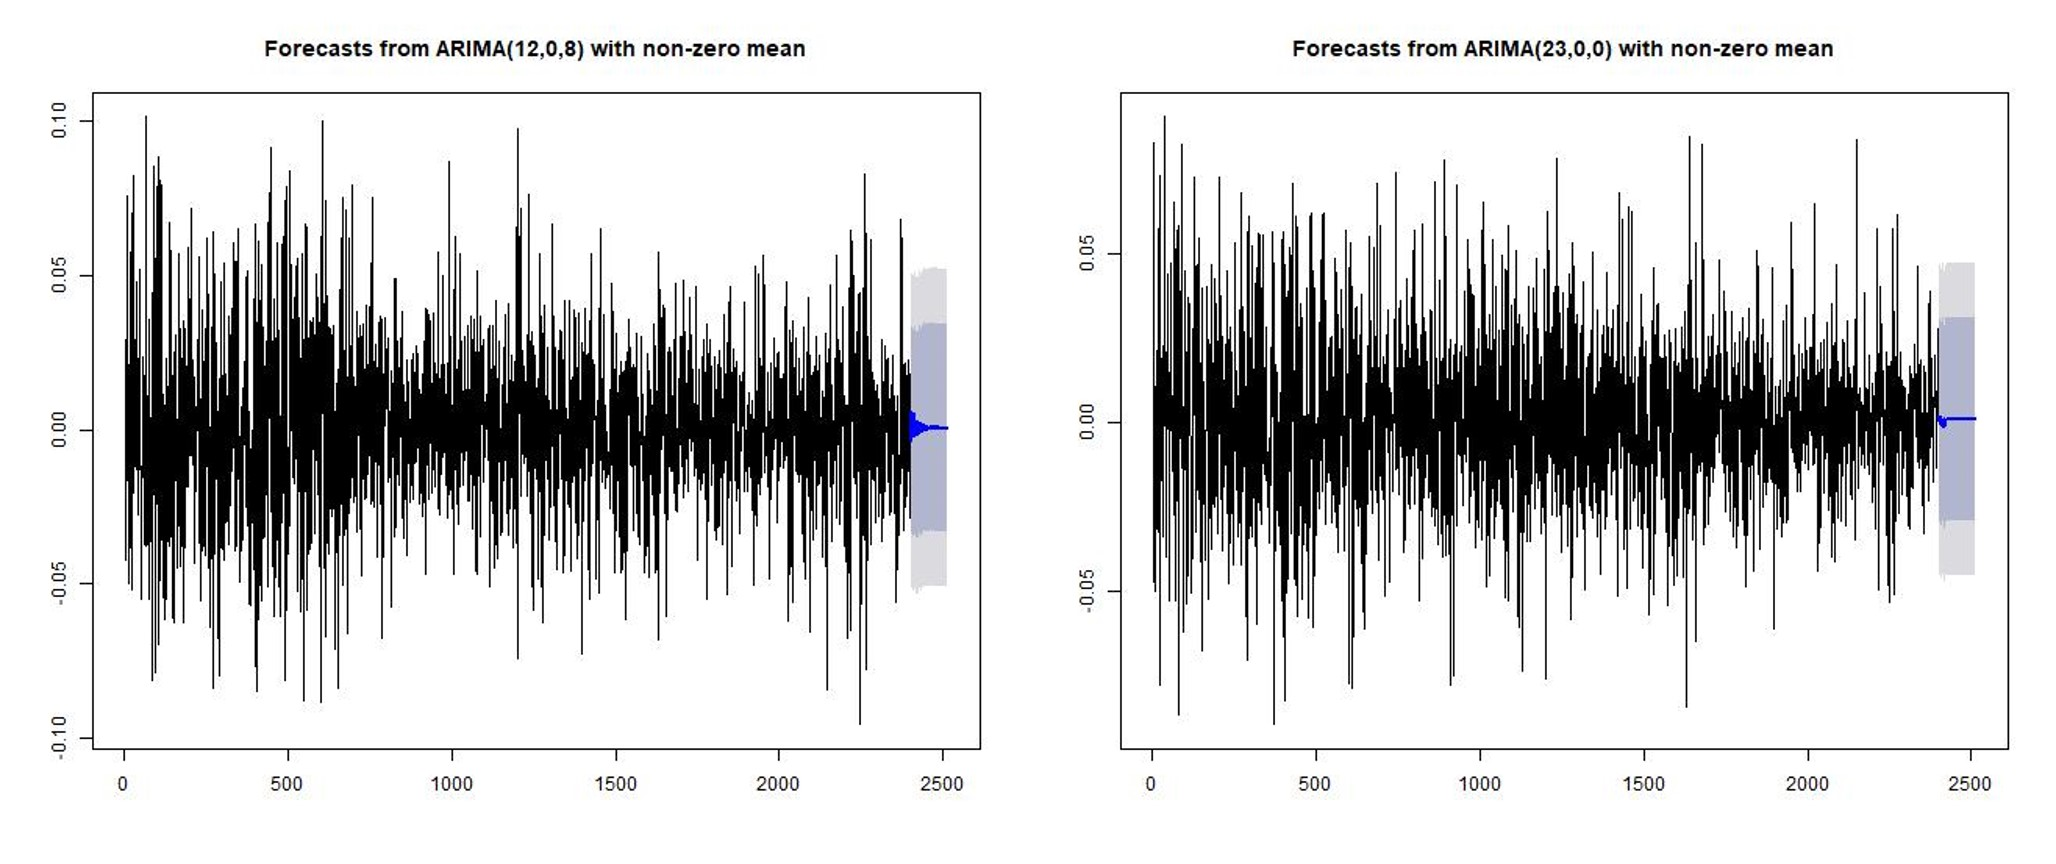
\includegraphics[width=0.9\linewidth]{../Modelos/ForecastAmerUnit}
	\caption{Forecast American e United}
	\label{fig:forecastamerunit}
\end{figure}
\begin{figure}[H]
	\centering
	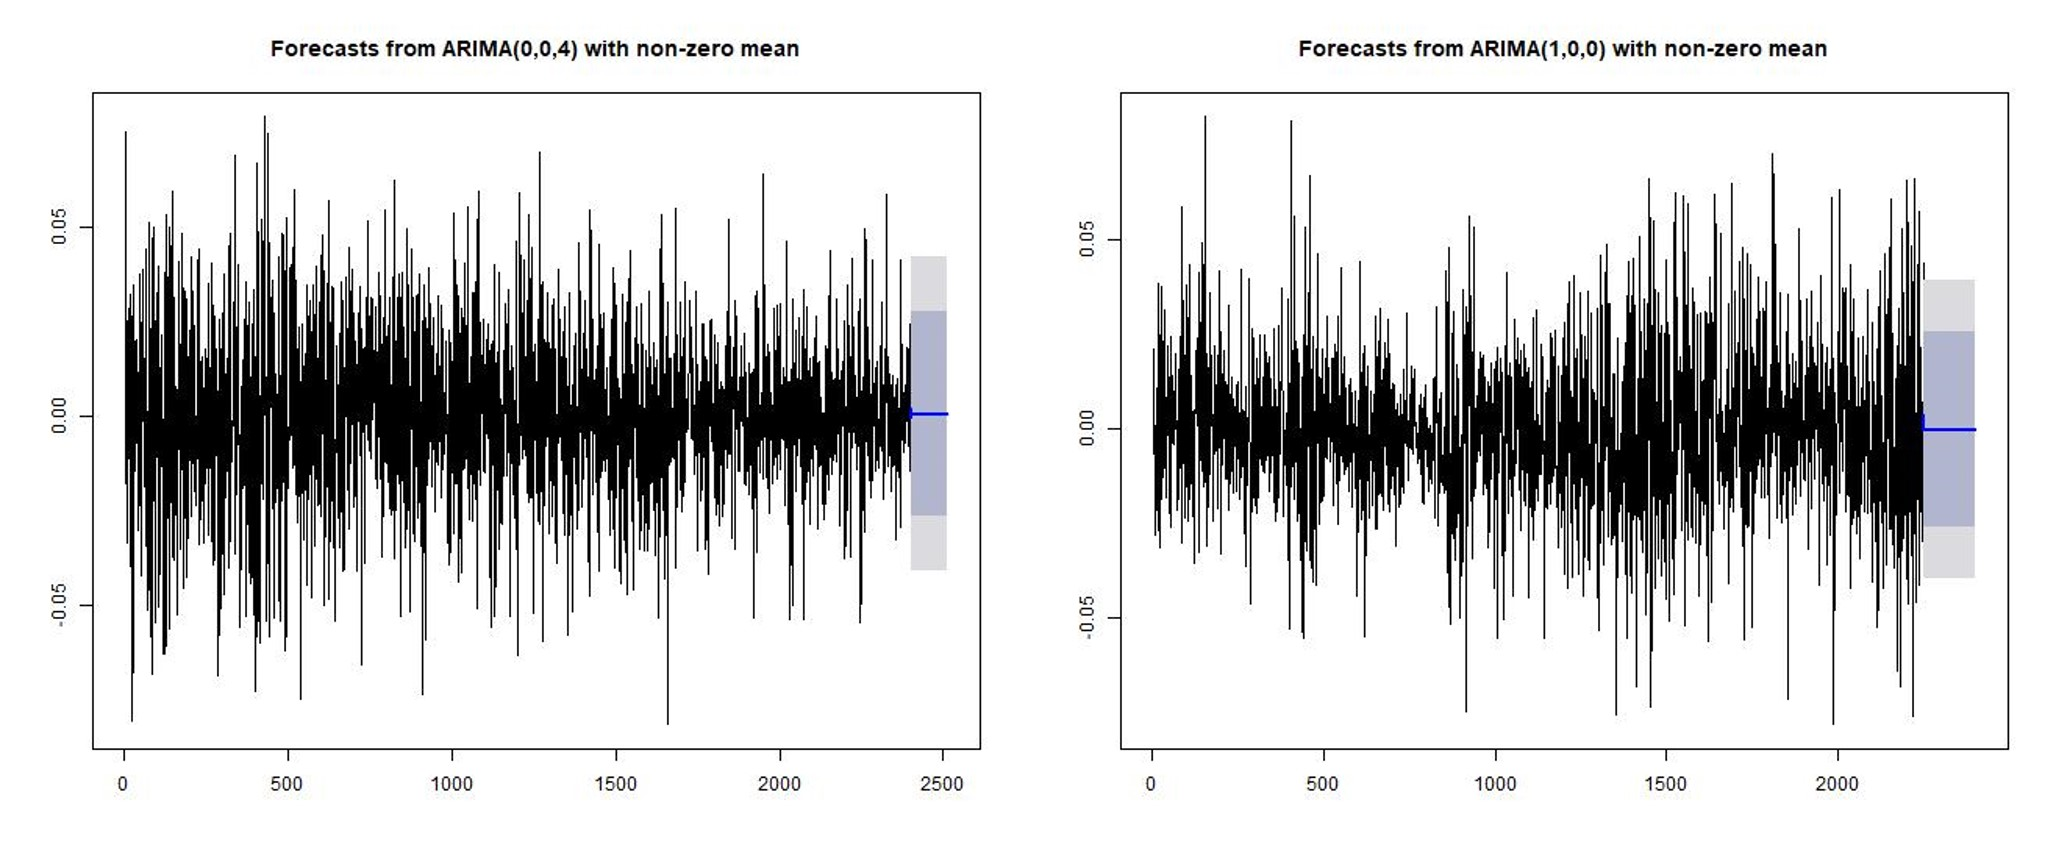
\includegraphics[width=0.9\linewidth]{../Modelos/ForecastDeltaLat}
	\caption{Forecast Delta e Latam}
	\label{fig:forecastdeltalat}
\end{figure}
\begin{figure}[H]
	\centering
	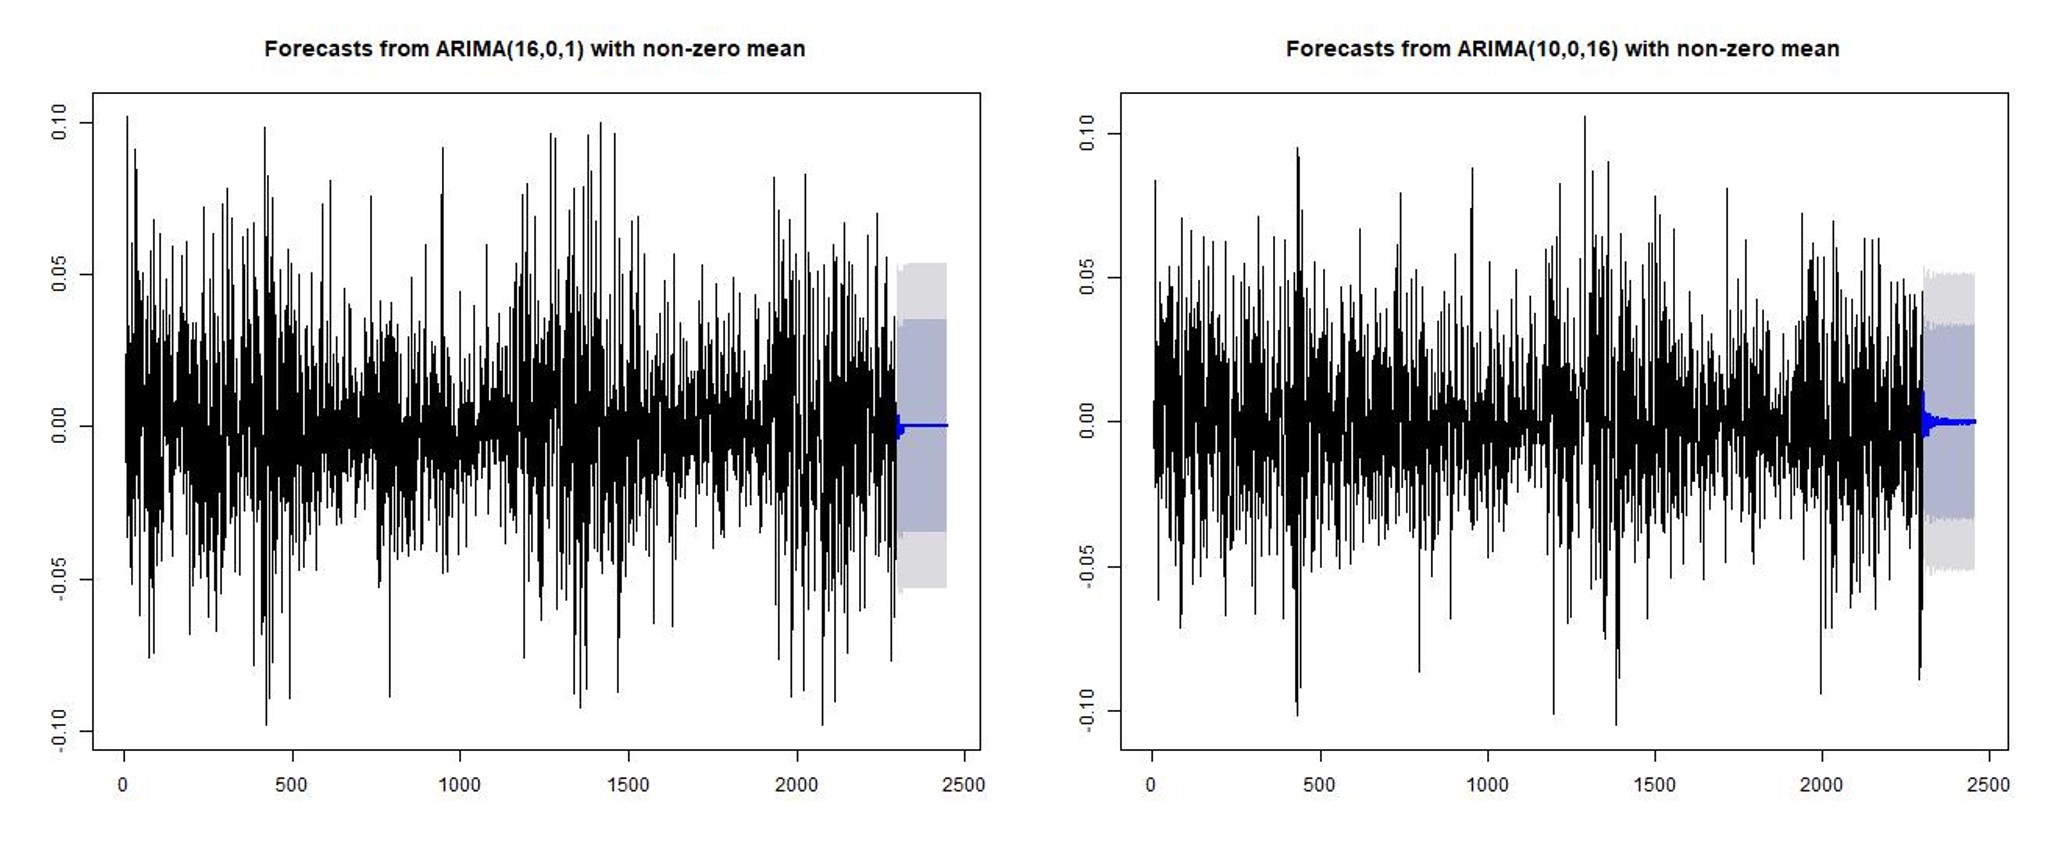
\includegraphics[width=0.9\linewidth]{../Modelos/ForecastChinaSoEast}
	\caption{Forecast China Southern e China Eastern}
	\label{fig:forecastchinasoeast}
\end{figure}
\begin{figure}[H]
	\centering
	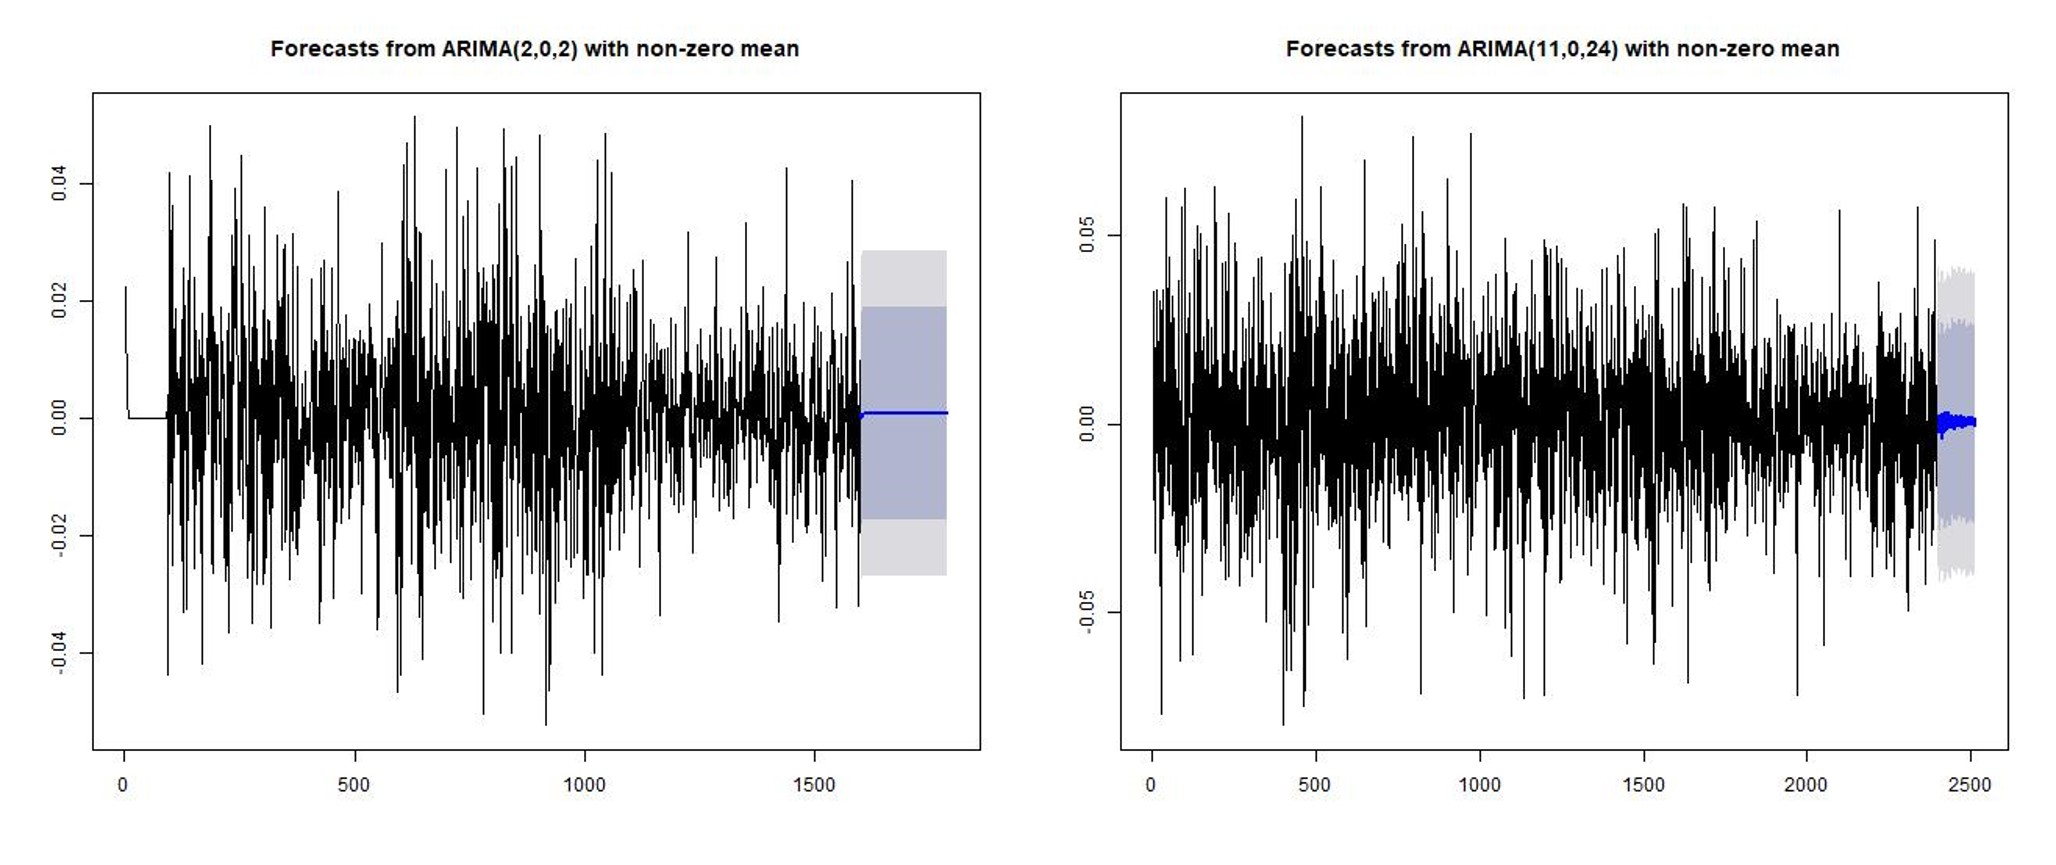
\includegraphics[width=0.9\linewidth]{../Modelos/ForecastJpIAG}
	\caption{Forecast Japan e IAG}
	\label{fig:forecastjpiag}
\end{figure}
\begin{figure}[H]
	\centering
	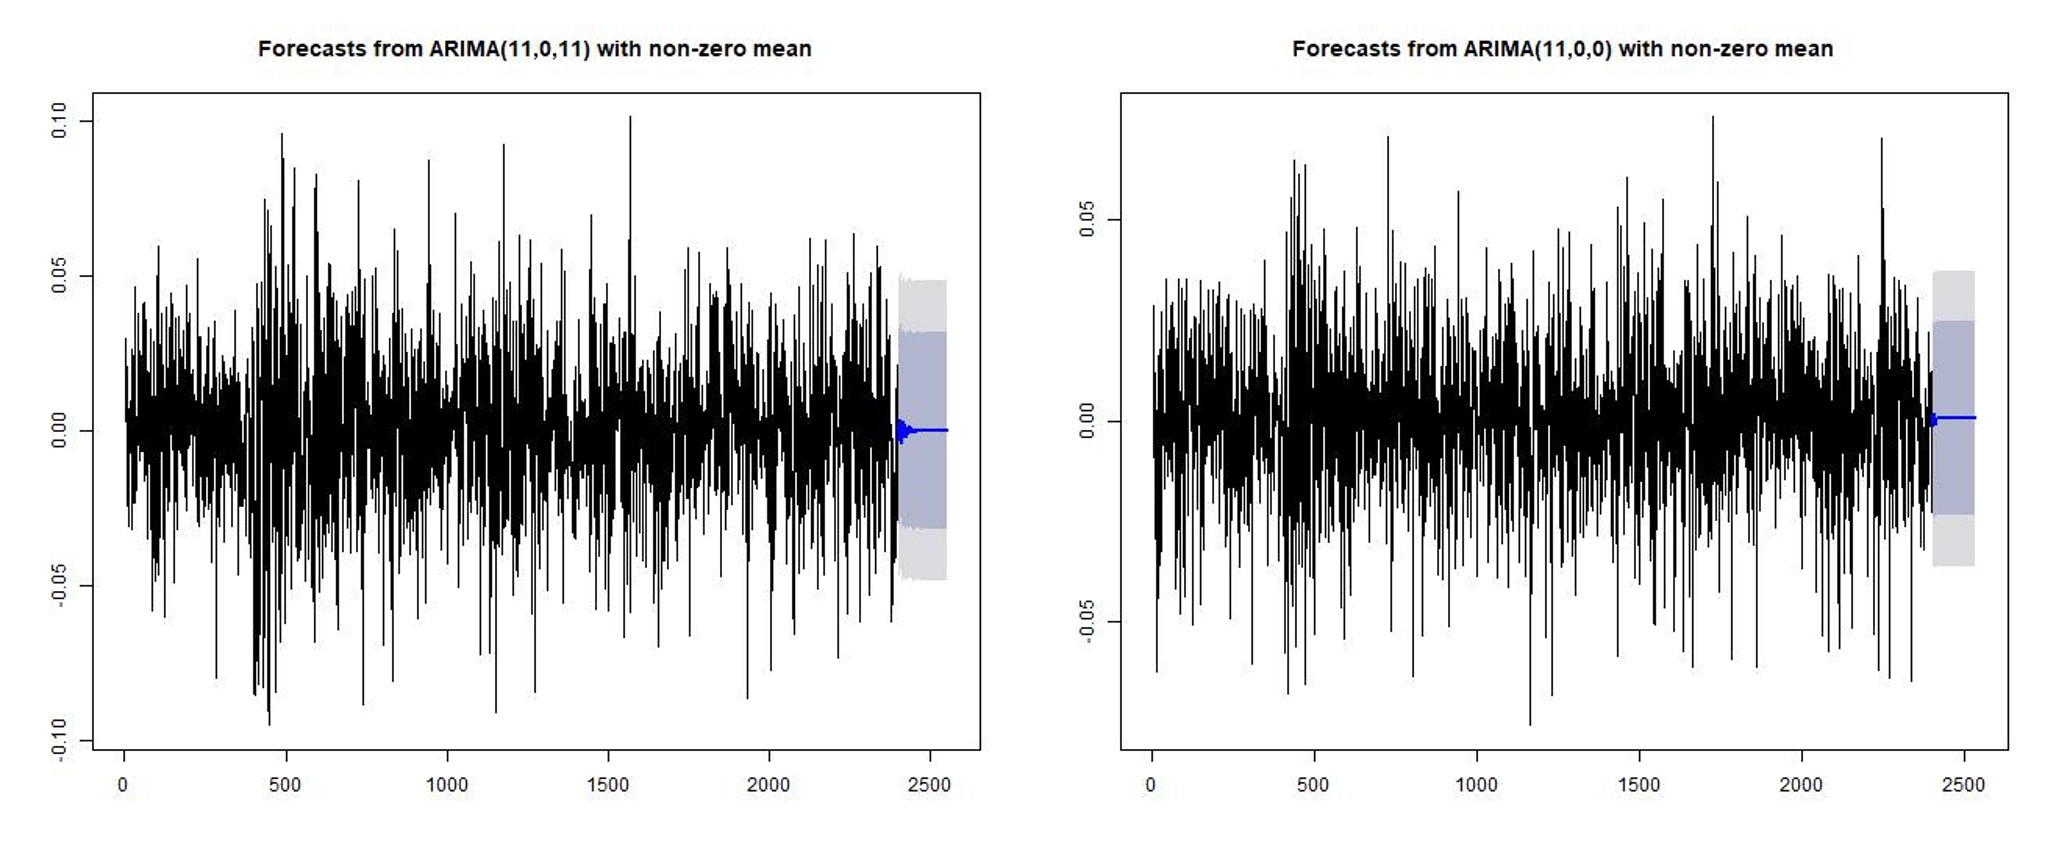
\includegraphics[width=0.9\linewidth]{../Modelos/ForecastKLMLuft}
	\caption{Forecast AirFrance-KLM e Lufthansa}
	\label{fig:forecastklmluft}
\end{figure}


Como critério de comparação, a fim de selecionar, enfim, o modelo cuja previsão apresenta a maior acurácia, foram utilizados os métodos apresentados na seção \ref{subsec_R}: $accuracy()$ e $checkresiduals()$. Com esse objetivo, dentre as várias medidas de erro fornecidas pela função $accuracy()$, optou-se por ter a \textit{RMSE - Root Mean Square Error} como medida de referência. Isso se justifica por seu caráter mais preciso, devido ao fato de utilizar a raiz quadrada do quadrado dos erros. Sendo assim, ao analisar o retorno desta função, procuramos o modelo cuja previsão \textit{(trainnig set)} possui o \textit{RMSE} menor e mais próximo possível da série de controle \textit{(testing set)}. O retorno da função $checkresiduals()$, por sua vez, deve ser analisado buscando-se a série residual menos auto-correlacionada, com média mais próxima de zero, maior perfil de estacionaridade e histograma similar à uma distribuição normal. As figuras e tabelas a seguir exibem esses resultados.

\begin{figure}[H]
	\centering
	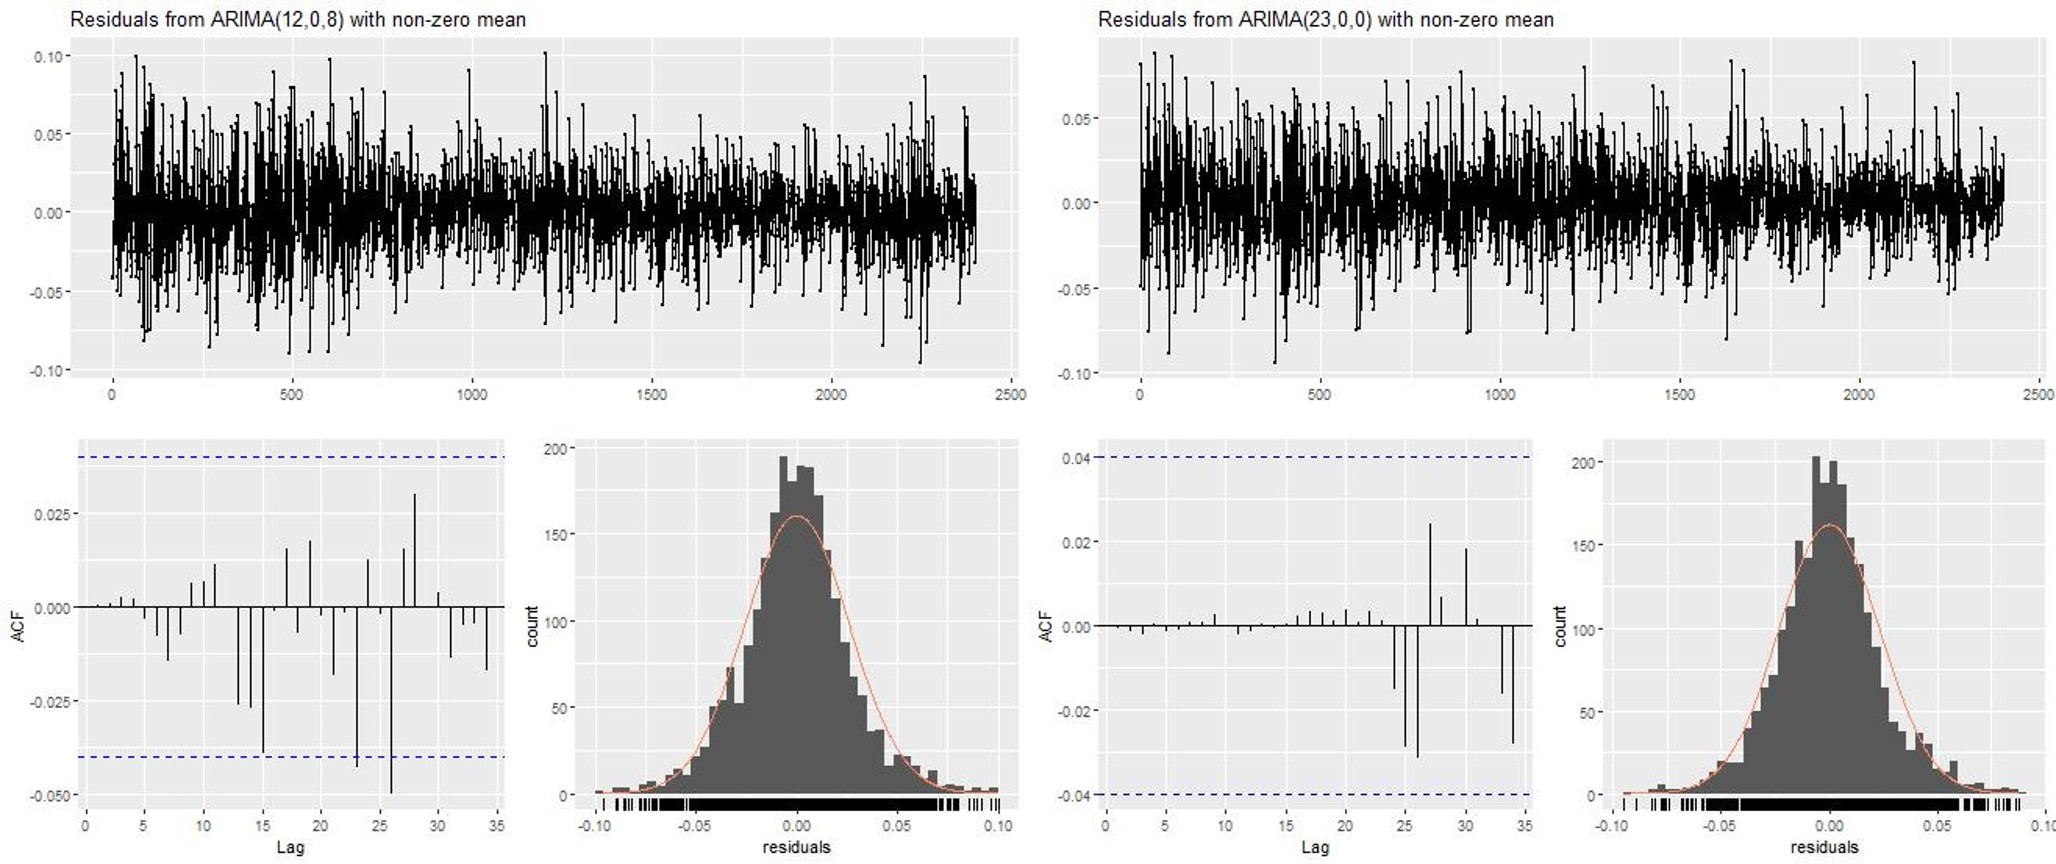
\includegraphics[width=1.0\linewidth]{../Modelos/ResidualsAmericanUnited}
	\caption{Checkresiduals American e United}
	\label{fig:residualsamericanunited}
\end{figure}
\begin{figure}[H]
	\centering
	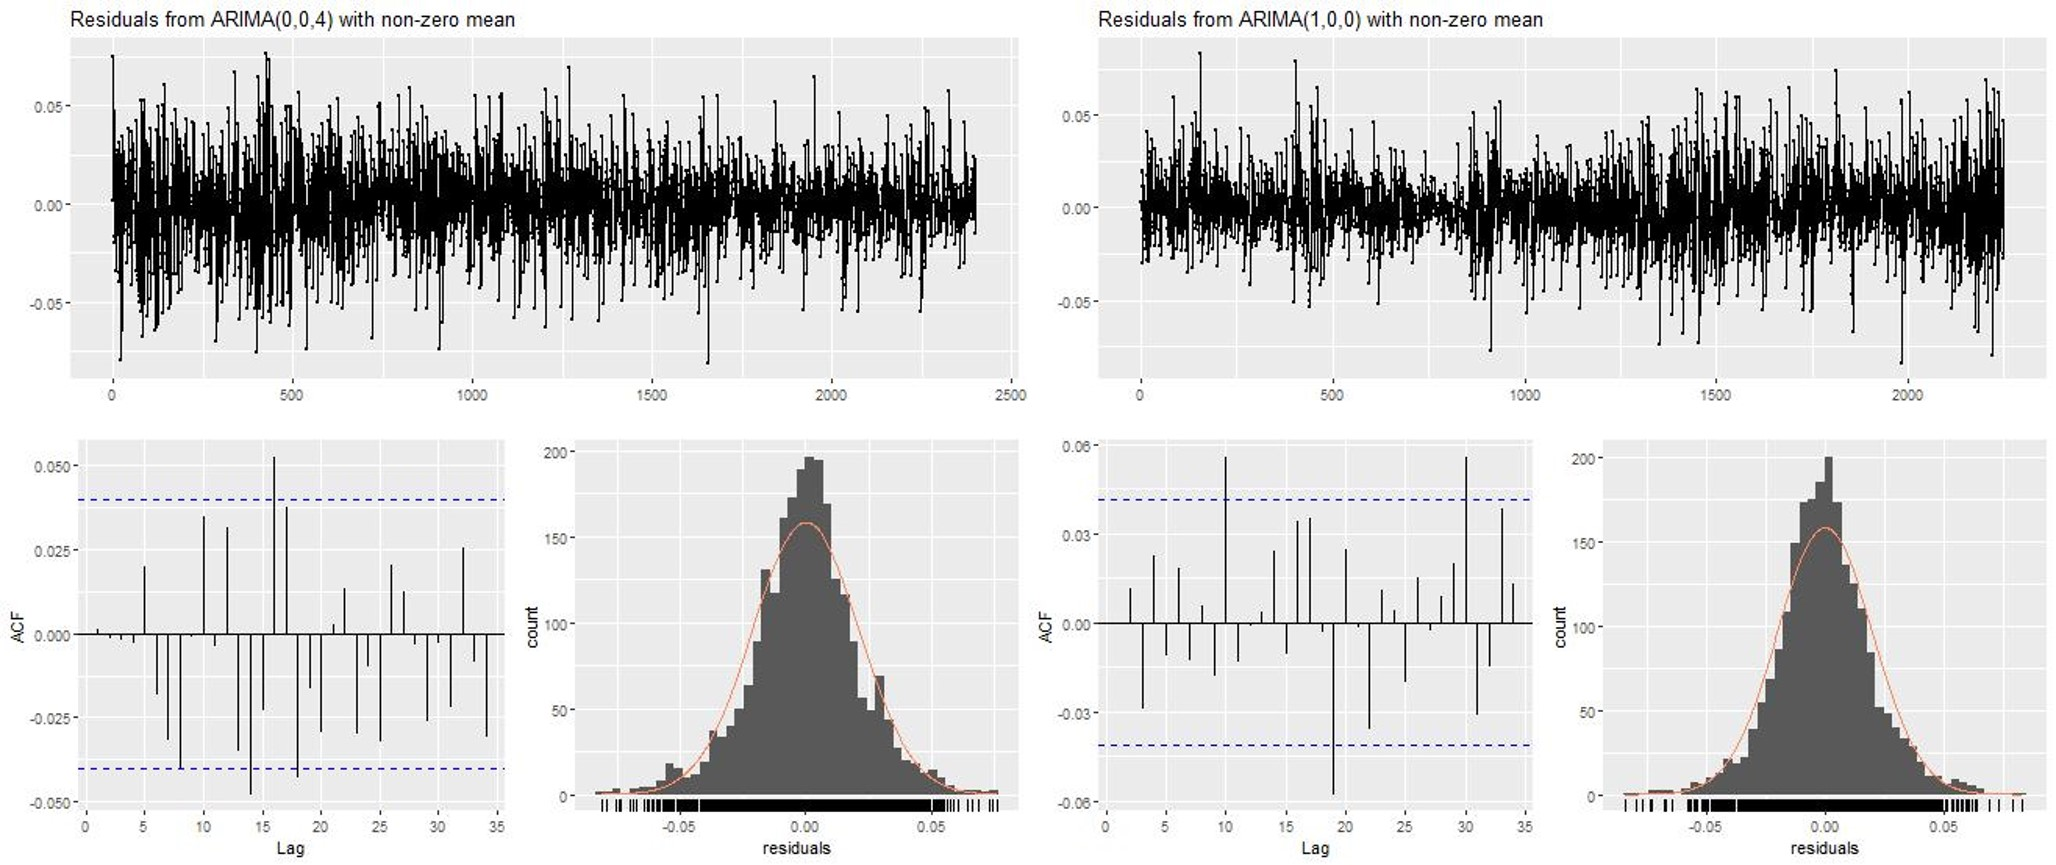
\includegraphics[width=1.0\linewidth]{../Modelos/ResidualsDeltaLatam}
	\caption{Checkresiduals Delta e Latam}
	\label{fig:residualsdeltalatam}
\end{figure}
\begin{figure}[H]
	\centering
	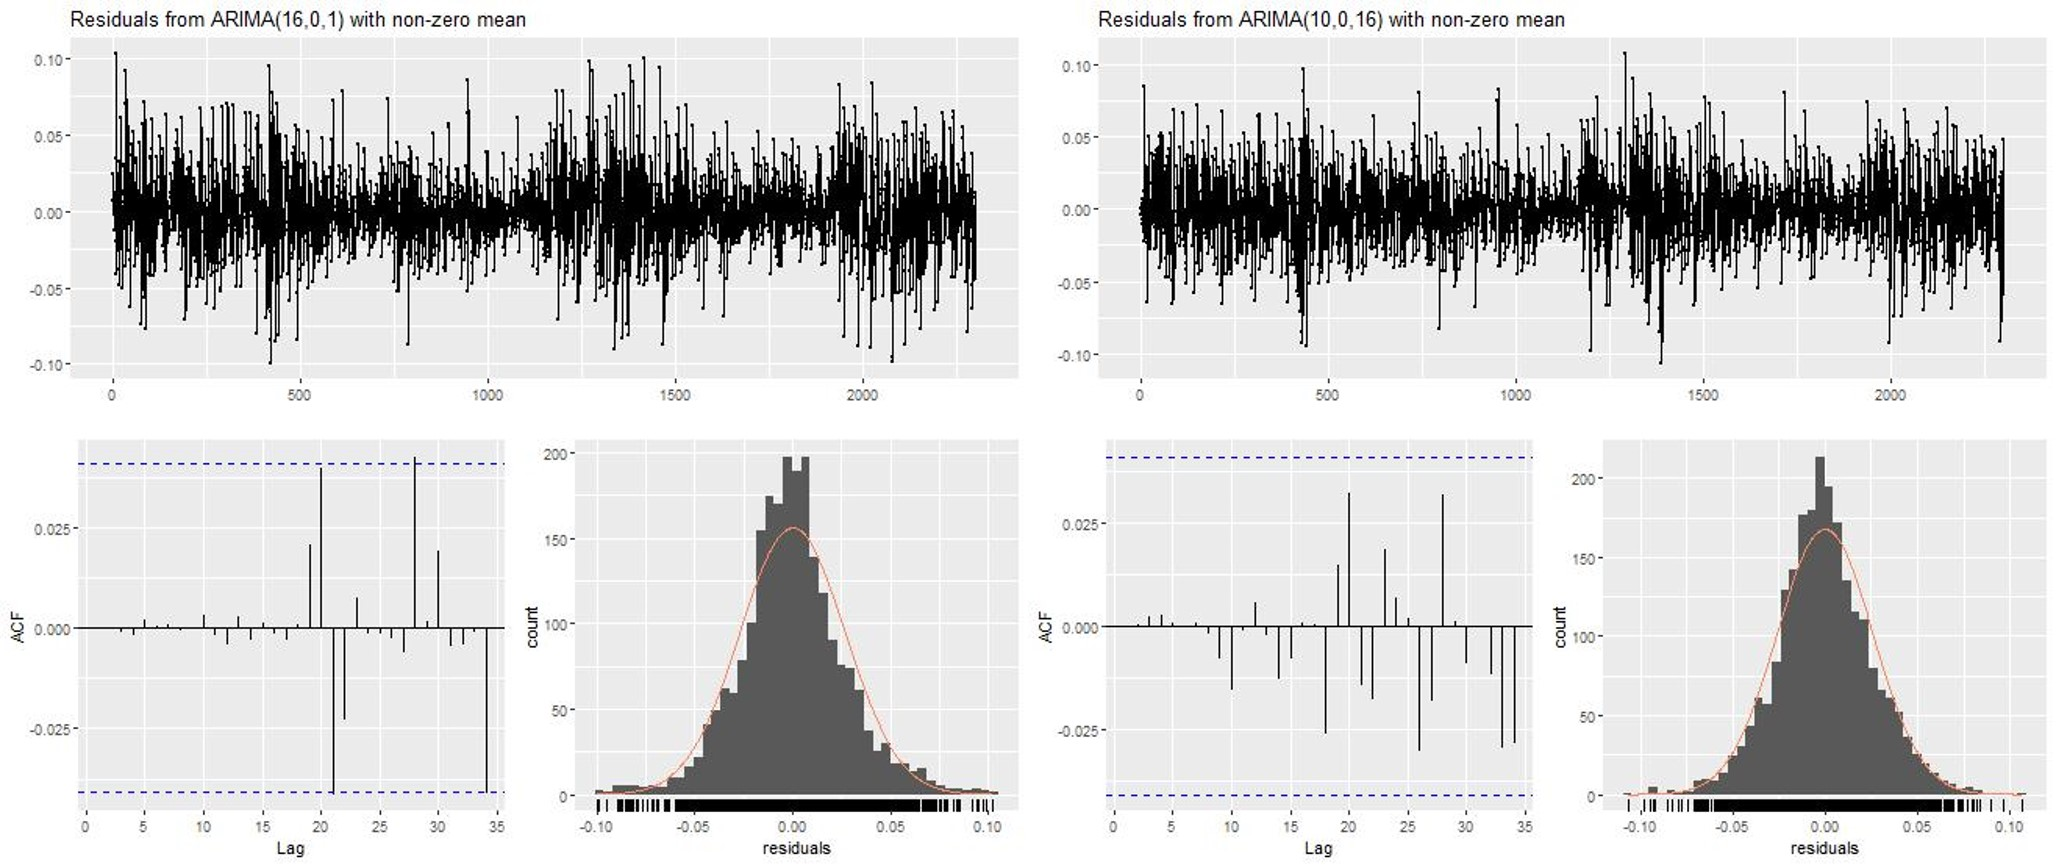
\includegraphics[width=1.0\linewidth]{../Modelos/ResidualsChinaSouEast}
	\caption{Checkresiduals China Southern e China Eastern}
	\label{fig:residualschinasoueast}
\end{figure}
\begin{figure}[H]
	\centering
	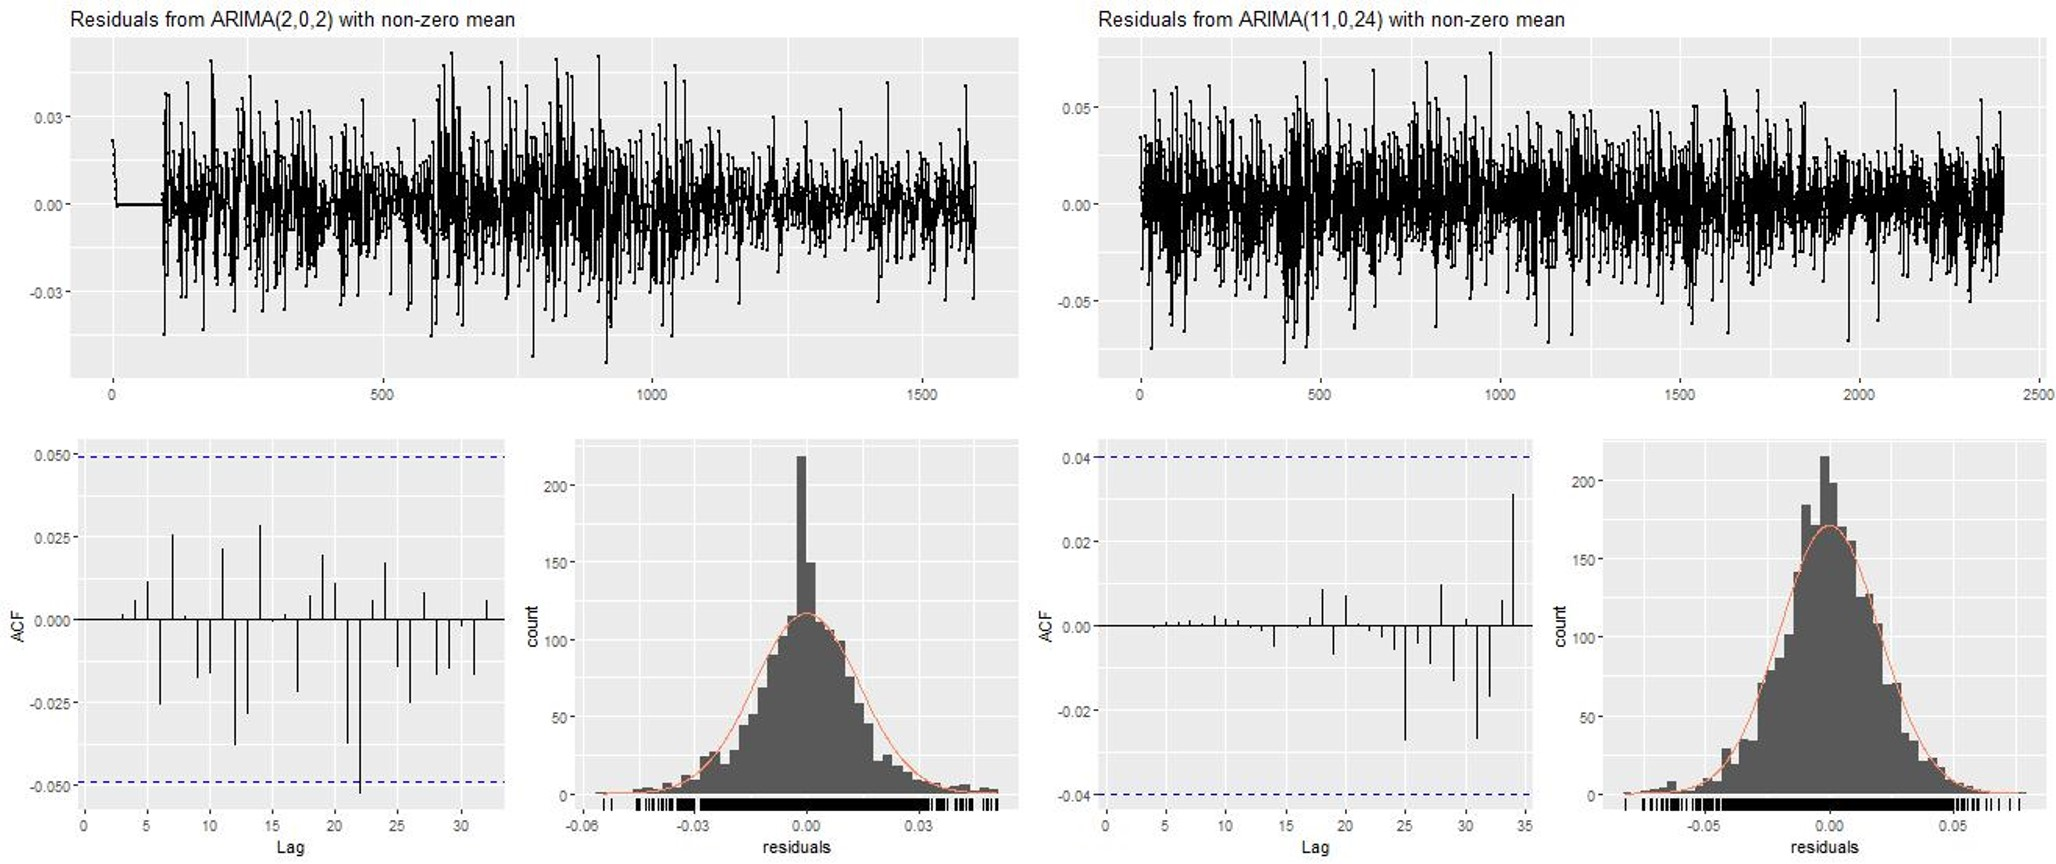
\includegraphics[width=1.0\linewidth]{../Modelos/ResidualsJapanIAG}
	\caption{Checkresiduals Japan e IAG}
	\label{fig:residualsjapaniag}
\end{figure}
\begin{figure}[H]
	\centering
	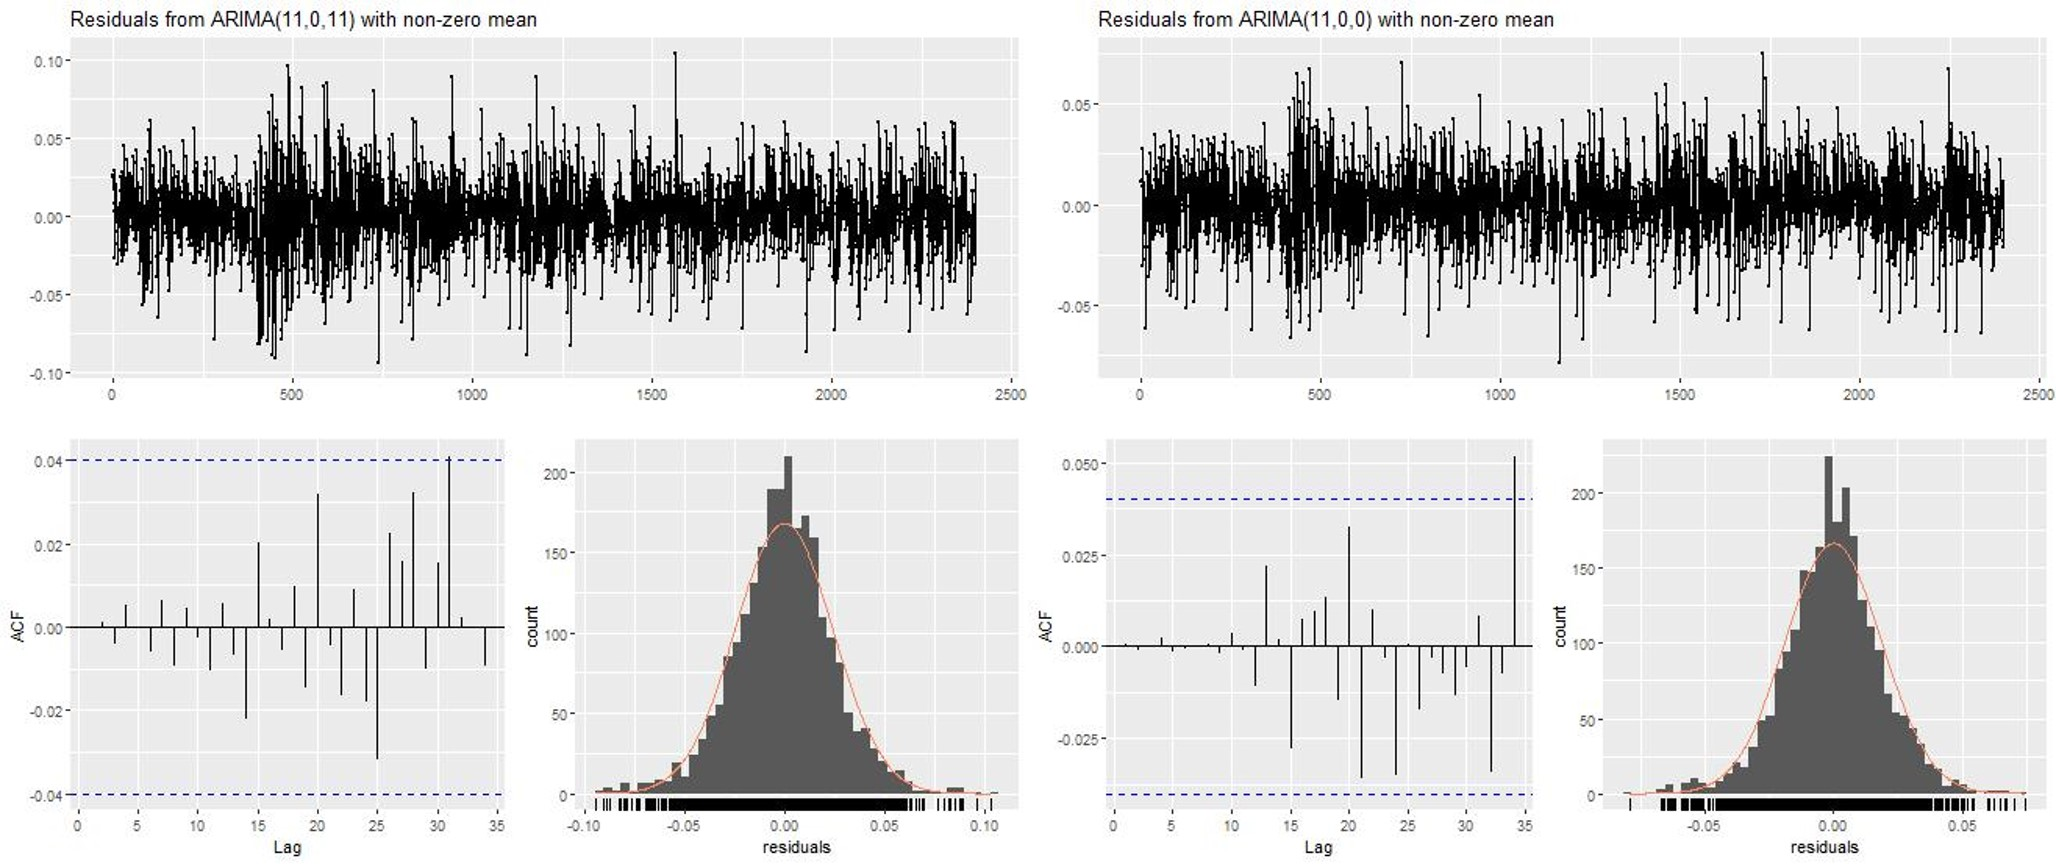
\includegraphics[width=1.0\linewidth]{../Modelos/ResidualsKLMLufthansa}
	\caption{Checkresiduals AirFrance-KLM e Lufthansa}
	\label{fig:residualsklmlufthansa}
\end{figure}

% Please add the following required packages to your document preamble:
% \usepackage{multirow}
\begin{table}[H]
	\centering
	\begin{tabular}{|l|l|l|l|l|}
		\cline{1-2} \cline{4-5}
		American (12,0,8) & RMSE       & \multirow{3}{*}{} & United (23,0,0) & RMSE       \\ \cline{1-2} \cline{4-5} 
		Training Set      & 0.02604072 &                   & Training Set    & 0.02342442 \\ \cline{1-2} \cline{4-5} 
		Test Set          & 0.02271122 &                   & Test Set        & 0.01319110 \\ \cline{1-2} \cline{4-5} 
	\end{tabular}
\label{tab:RMSEAmerican}
\caption{RMSE American e United}
\end{table}

\begin{table}[H]
	\centering
	\begin{tabular}{|l|l|l|l|l|}
		\cline{1-2} \cline{4-5}
		Delta (0,0,4) & RMSE       & \multirow{3}{*}{} & Latam (1,0,0) & RMSE       \\ \cline{1-2} \cline{4-5} 
		Training Set  & 0.02119129 &                   & Training Set  & 0.02009249 \\ \cline{1-2} \cline{4-5} 
		Test Set      & 0.01307335 &                   & Test Set      & 0.02029929 \\ \cline{1-2} \cline{4-5} 
	\end{tabular}
\label{tab:RMSEDelta}
\caption{RMSE Delta e Latam}
\end{table}

\begin{table}[H]
	\centering
	\begin{tabular}{|l|l|l|l|l|}
		\cline{1-2} \cline{4-5}
		China Southern (16,0,1) & RMSE       & \multirow{3}{*}{} & China Eastern (10,0,16) & RMSE       \\ \cline{1-2} \cline{4-5} 
		Training Set            & 0.02700575 &                   & Training Set            & 0.02601087 \\ \cline{1-2} \cline{4-5} 
		Test Set                & 0.02004664 &                   & Test Set                & 0.02116064 \\ \cline{1-2} \cline{4-5} 
	\end{tabular}
\label{tab:RMSEChina}
\caption{RMSE China Southern e China Eastern}
\end{table}

\begin{table}[H]
	\centering
	\begin{tabular}{|l|l|l|l|l|}
		\cline{1-2} \cline{4-5}
		Japan (2,0,2) & RMSE       & \multirow{3}{*}{} & IAG (11,0,24) & RMSE       \\ \cline{1-2} \cline{4-5} 
		Training Set  & 0.01408789 &                   & Training Set  & 0.02021170 \\ \cline{1-2} \cline{4-5} 
		Test Set      & 0.01165704 &                   & Test Set      & 0.01997025 \\ \cline{1-2} \cline{4-5} 
	\end{tabular}
\label{tab:RMSEJapan}
\caption{RMSE Japan e IAG}
\end{table}

\begin{table}[H]
	\centering
	\begin{tabular}{|l|l|l|l|l|}
		\cline{1-2} \cline{4-5}
		AirFrance-KLM (11,0,11) & RMSE       & \multirow{3}{*}{} & Lufthansa (11,0,0) & RMSE       \\ \cline{1-2} \cline{4-5} 
		Training Set            & 0.02450562 &                   & Training Set       & 0.01878714 \\ \cline{1-2} \cline{4-5} 
		Test Set                & 0.01983093 &                   & Test Set           & 0.01680258 \\ \cline{1-2} \cline{4-5} 
	\end{tabular}
\label{tab:RMSEKLM}
\caption{RMSE AirFrance-KLM e Lufthansa}
\end{table}

Enfim, chegamos ao melhor modelo de cada companhia aérea, tendo como base a comparação dos diversos resultados comentados e exibidos anteriormente. São eles: \emph{\textbf{American} - (12,0,8); \textbf{United} - (23,0,0); \textbf{Delta} - (0,0,4); \textbf{Latam} - (1,0,0); \textbf{China Southern} - (16,0,1); \textbf{China Eastern} - (10,0,16); \textbf{Japan} - (2,0,2); \textbf{IAG} - (11,0,24); \textbf{AirFranceKLM} - (11,0,11); e \textbf{Lufthansa} - (11,0,0)}. Após toda esta análise e aplicação dos conceitos teóricos estudados na seção \ref{subsec_teoria}, podemos observar alguns fatos interessantes sobre a modelagem econométrica clássica, começando por dois grandes comentários acerca das figuras \ref{fig:forecastamerunit} a \ref{fig:forecastklmluft}. Primeiramente, para o intervalo de confiança escolhido, as previsões se mostram um pouco frouxas, no sentido de que os retornos previstos pela modelagem $ARIMA$ dentro de 80-95\% de confiança podem assumir, praticamente, qualquer valor dentro da amplitude da série de retornos, o que é evidenciado pelos limites inferior e superior das faixas cinzas. Somado a isso, nota-se que a qualidade da precisão decai consideravelmente com o aumento do número de passos futuros previstos, o que é percebido pela tendência da curva azul, isto é, dos valores previstos, aproximarem-se de zero em todos os modelos ajustados. Tal caráter poderia ser fruto de modelos mal ajustados. Contudo, ao analisarmos os resíduos exibidos nas figuras \ref{fig:residualsamericanunited} a \ref{fig:residualsklmlufthansa}, essa suposição parece ser negada, pois diversas características desejáveis são percebidas nas imagens, sejam funções $ACF$ sem \textit{lags} significativos, distribuição próxima à normal ou médias próximas de zero. Desse modo, tal fato parece decorrer das próprias limitações dos modelos $ARIMA$.

\section{Conclusões}
Como discutido na seção anterior, a modelagem $ARIMA$ apresenta-se como uma ferramenta extremamente poderosa para o estudo e compreensão de séries temporais aplicadas no contexto financeiro. Isso se justifica por todos os conceitos teóricos cujo entendimento é necessário para a plena aplicação e compreensão deste modelo. Além de todo o amplo conhecimento pré-requisito para a formulação deste trabalho, cujo objetivo é a previsão de séries temporais, a modelagem $ARIMA$ mostra-se útil em alguns contextos plausíveis da realidade. Tome por exemplo um investidor que pretende escolher entre algumas empresas aquela mais confiável de se tornar fim de seu investimento. Caso esta pessoa preocupe-se em especial com a evolução de curto prazo dos retornos dos ativos, utilizar uma aplicação que ajuste modelos $ARIMA$ para dados históricos das empresas e preveja, dentro de um intervalo de confiança confortável, esse desenvolvimento, seria uma estratégia muito interessante. Por outro lado, para fins de análise a longo prazo, a modelagem $ARIMA$ revela-se pouco adequada, justificado pelas conclusões discutidas na seção \ref{subsec_for}. Desse modo, outras ferramentas da econometria de séries financeiras devem mostra-se mais confiáveis. O estudo da teoria das \emph{ondaletas}, objetivo futuro e passo seguinte desta pesquisa, talvez apresente-se, de fato, como uma evolução mais poderosa e generalizada da modelagem clássica aqui abordada.

\bibliographystyle{amsplain, amsalpha}
\begin{thebibliography}{99} 
	
	\bibitem{Tsay} R. S. Tsay,
	{\bf Analysis of financial time series},
	Third edition. Wiley Series in Probability and Statistics. {\it John Wiley \& Sons, Inc., Hoboken, NJ.}  (2010).
	
	\bibitem{Tsay-Tiao1984} R. S. Tsay and G. C. Tiao,
	{\it Consistent estimates of autoregressive parameters and extended sample autocorrelation function for stationary and nonstationary ARMA models},
	J. Amer. Statist. Assoc. 79, p.84-96 (1984).
	
	\bibitem{CRANR} 
	CRAN R Project, \texttt{https://cran.r-project.org/}
	
	\bibitem{git} 
	Github Repository, \texttt{https://github.com/MathNog/UndergraduateResearchProject.git}
	
\end{thebibliography}
\end{document}

